%!TEX root = ../nwoods_thesis.tex

\chapter{Results}

A number of measurements and analyses fall under the umbrella of four-lepton physics, and results of the work presented in this thesis were presented in several journal articles and Physics Analysis Summary documents made public by the CMS collaboration.
The first CMS measurement of the {\ZZ} inclusive cross section at {13\TeV} used roughly half the 2015 dataset ({1.34\fbinv}) and was presented in Ref.~\cite{CMS:2015fnj}.
That analysis was expanded to use the whole {2.6\fbinv} collected in 2015, and to include the {\Zfourl} branching fraction measurement, as we reported in Ref.~\cite{Khachatryan:2016txa}.
With the full 2016 dataset, the {\ZZ} cross section and {\Zfourl} branching ratio were measured again to greater precision in Ref.~\cite{CMS:2017ruh}, which also included differential cross section measurements and aTGC limits.
An upcoming paper including these measurements will also include a combination of the 2015 and 2016 inclusive cross section measurements.
Differential cross sections with respect to jet-related observables, and searches for EWK {\ZZ} production and aTGCs, were reported in Ref.~\cite{CMS:2017dyw}, which will be split into two papers (one for the cross section measurements, one for the searches) for final journal publication.
The Higgs boson was studied in the four-lepton final state in Refs.~\cite{CMS:2016rqf,CMS:2016ilx,Sirunyan:2017exp}.
In the following, results for each topic are only shown for 2016 data, which are taken to supersede 2015 data.



\section{Four-Lepton Yield and Distributions}


\subsection{Full Spectrum}

The full four-lepton invariant mass spectrum is shown in Fig.~\ref{fig:mass_full}.
The single-{\PZ} resonance can be seen below {100\GeV}, the Higgs resonance is visible---though unresolved with this binning---in the {\Zgs} region below $2m_\PZ$, where the doubly resonant {\ZZ} continuum begins.
The dilepton invariant mass spectrum is shown for both {\Zgs} candidates in Fig.~\ref{fig:zMass_full} and for the {\Zgs} candidate closest to the nominal {\PZ} boson mass ($\PZ_1$) in Fig.~\ref{fig:z1Mass_full}.
Figure~\ref{fig:mZ2VsmZ1_full} shows $m_{\PZ_2}$ plotted against $m_{\PZ_1}$ for data events representative of all four-lepton production.
Clusters of events with zero ({\Zfourl} and nonresonant $\Pa^\ast \Pa^\ast$ production), one ($\PH \to \PZ\PZ^\ast$ and nonresonant $\PZ\Pa^\ast$ production), and two (nonresonant {\ZZ} production) on-shell {\PZ} bosons can be clearly seen.

\begin{figure}[htbp]
  \begin{center}
    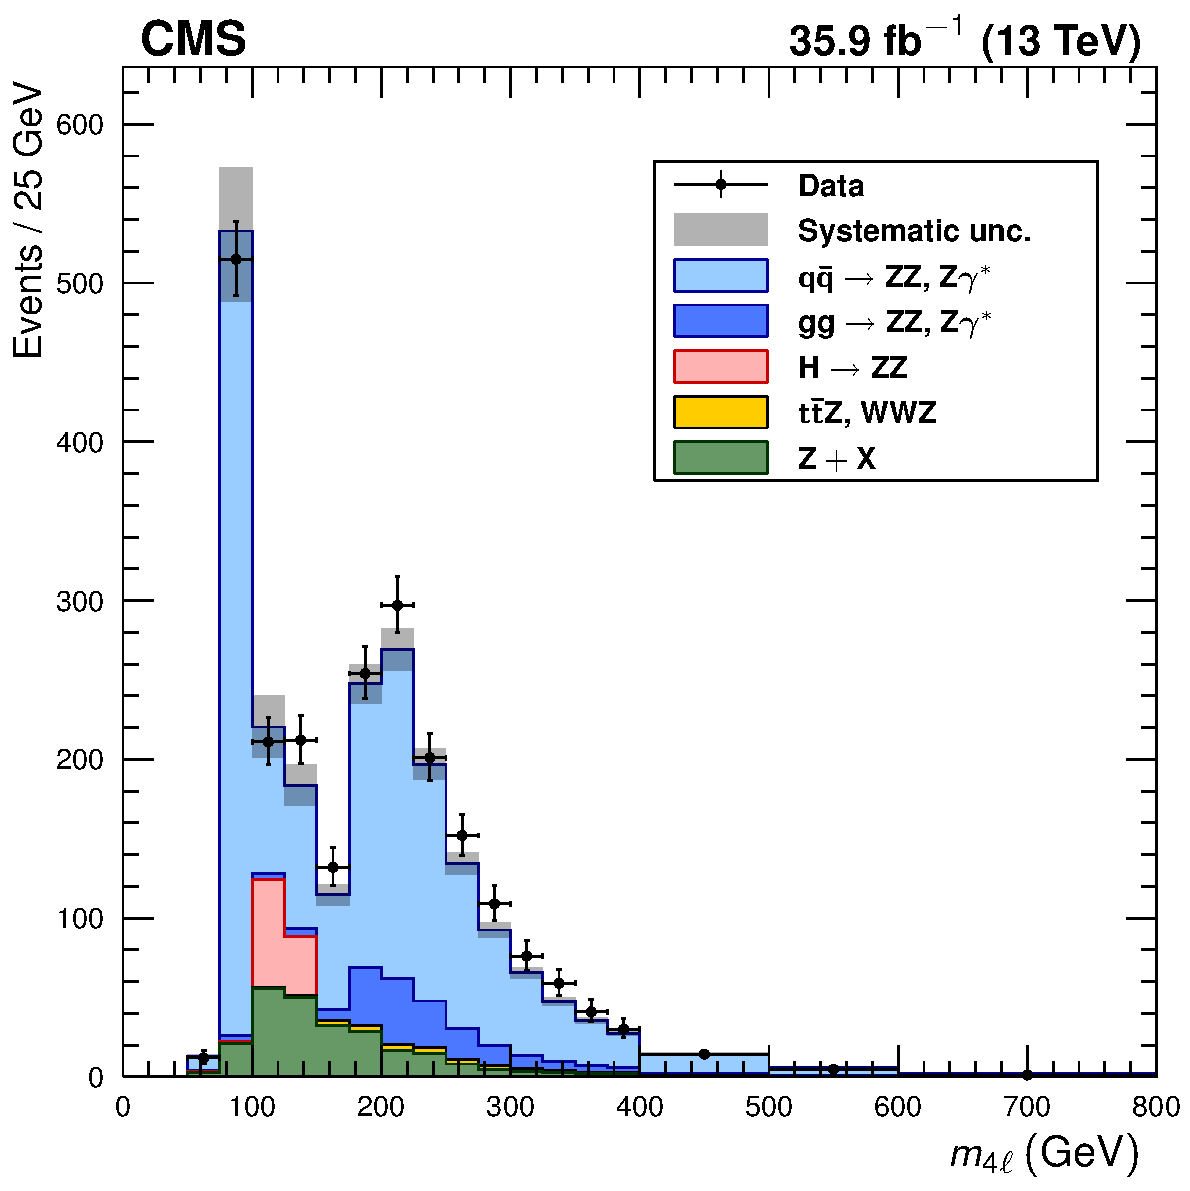
\includegraphics[width=0.75\textwidth]{results/zzMass.pdf}
    \caption[Full four-lepton mass spectrum]{
        Distribution of the four-lepton invariant mass $m_{4\ell}$ of all events in the full spectrum selection.
        Points represent data, with statistical uncertainty bars.
        The stack of filled histograms represents the SM signal prediction and background estimate, with a grey band showing the sum in quadrature of the statistical and systematic uncertainties on the total expected yield.
      }\label{fig:mass_full}
  \end{center}
\end{figure}

\begin{figure}[htbp]
  \begin{center}
    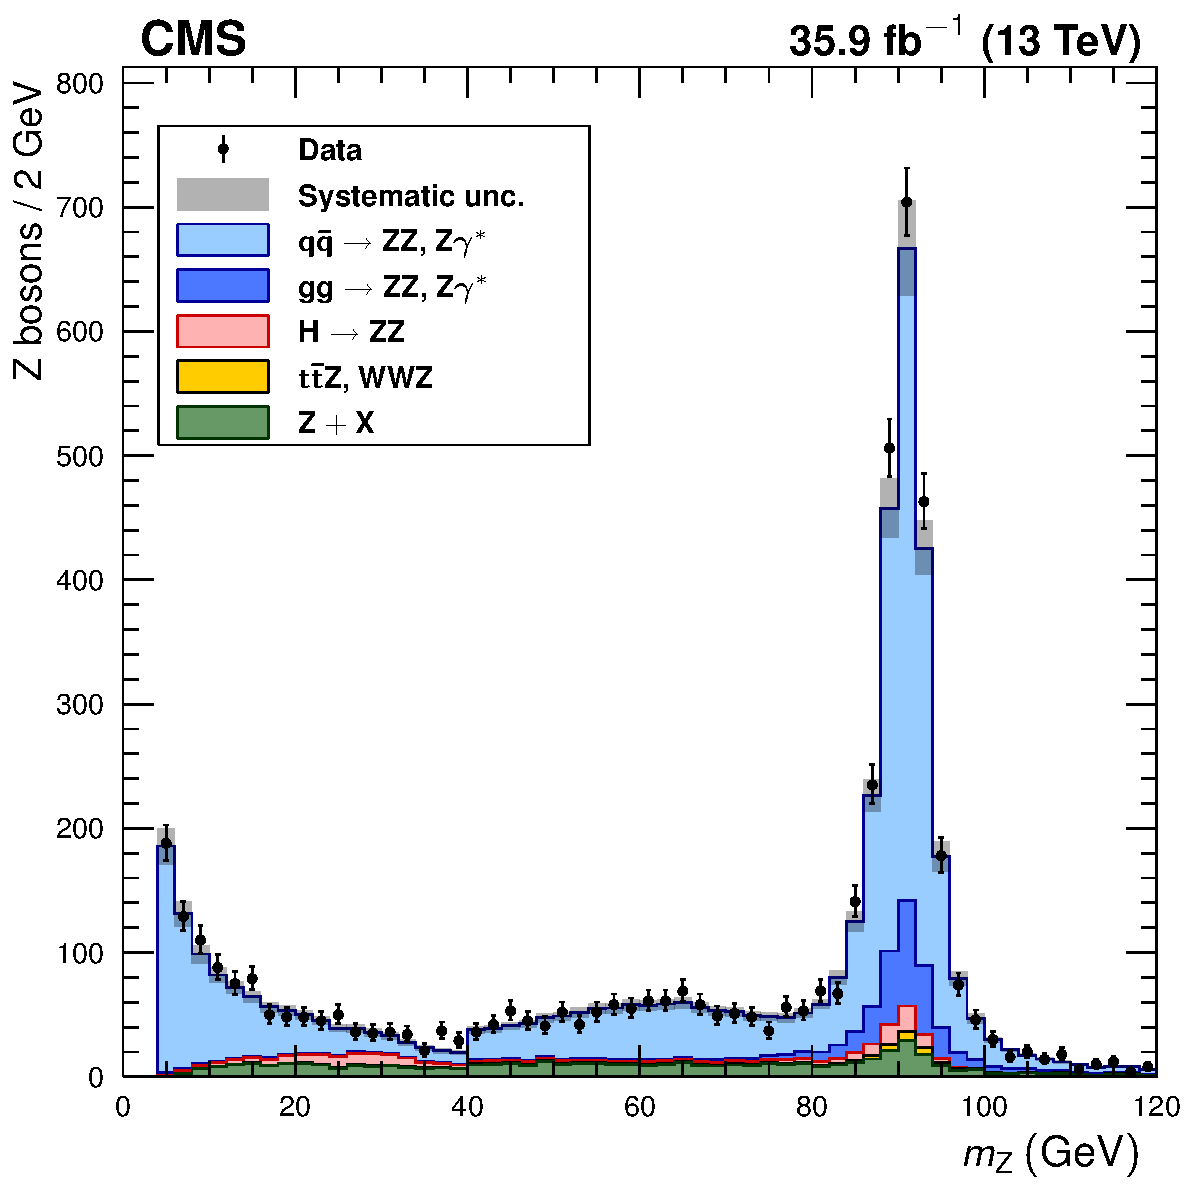
\includegraphics[width=0.75\textwidth]{results/zMass.pdf}
    \caption[Mass of all {\Zgs} candidates in the full spectrum selection]{
        Distribution of the dilepton invariant mass of {\Zgs} candidates in all events in the full spectrum selection, regardless of whether the lepton pair is labeled $\PZ_1$ or $\PZ_2$.
        Points represent data, with statistical uncertainty bars.
        The stack of filled histograms represents the SM signal prediction and background estimate, with a grey band showing the sum in quadrature of the statistical and systematic uncertainties on the total expected yield.
      }\label{fig:zMass_full}
  \end{center}
\end{figure}

\begin{figure}[htbp]
  \begin{center}
    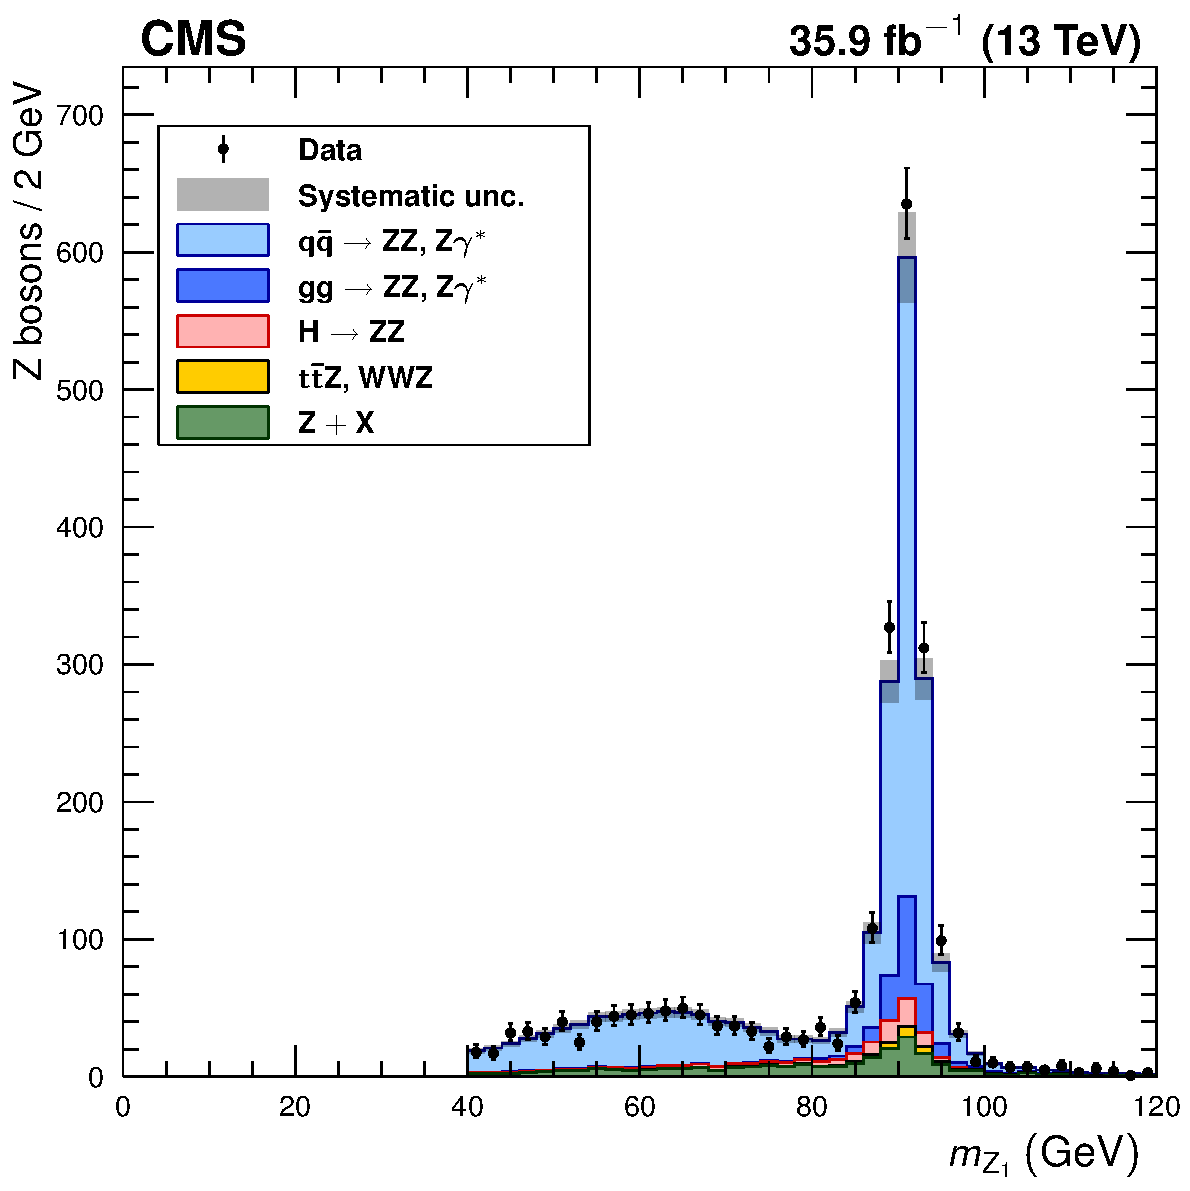
\includegraphics[width=0.75\textwidth]{results/z1Mass.pdf}
    \caption[Mass of $\PZ_1$ candidates in the full spectrum selection]{
        Distribution of the dilepton invariant mass of $\PZ_1$, the {\Zgs} candidate in each event closest to the nominal $m_\PZ$, in the full spectrum selection.
        Points represent data, with statistical uncertainty bars.
        The stack of filled histograms represents the SM signal prediction and background estimate, with a grey band showing the sum in quadrature of the statistical and systematic uncertainties on the total expected yield.
      }\label{fig:z1Mass_full}
  \end{center}
\end{figure}

\begin{figure}[htbp]
  \begin{center}
    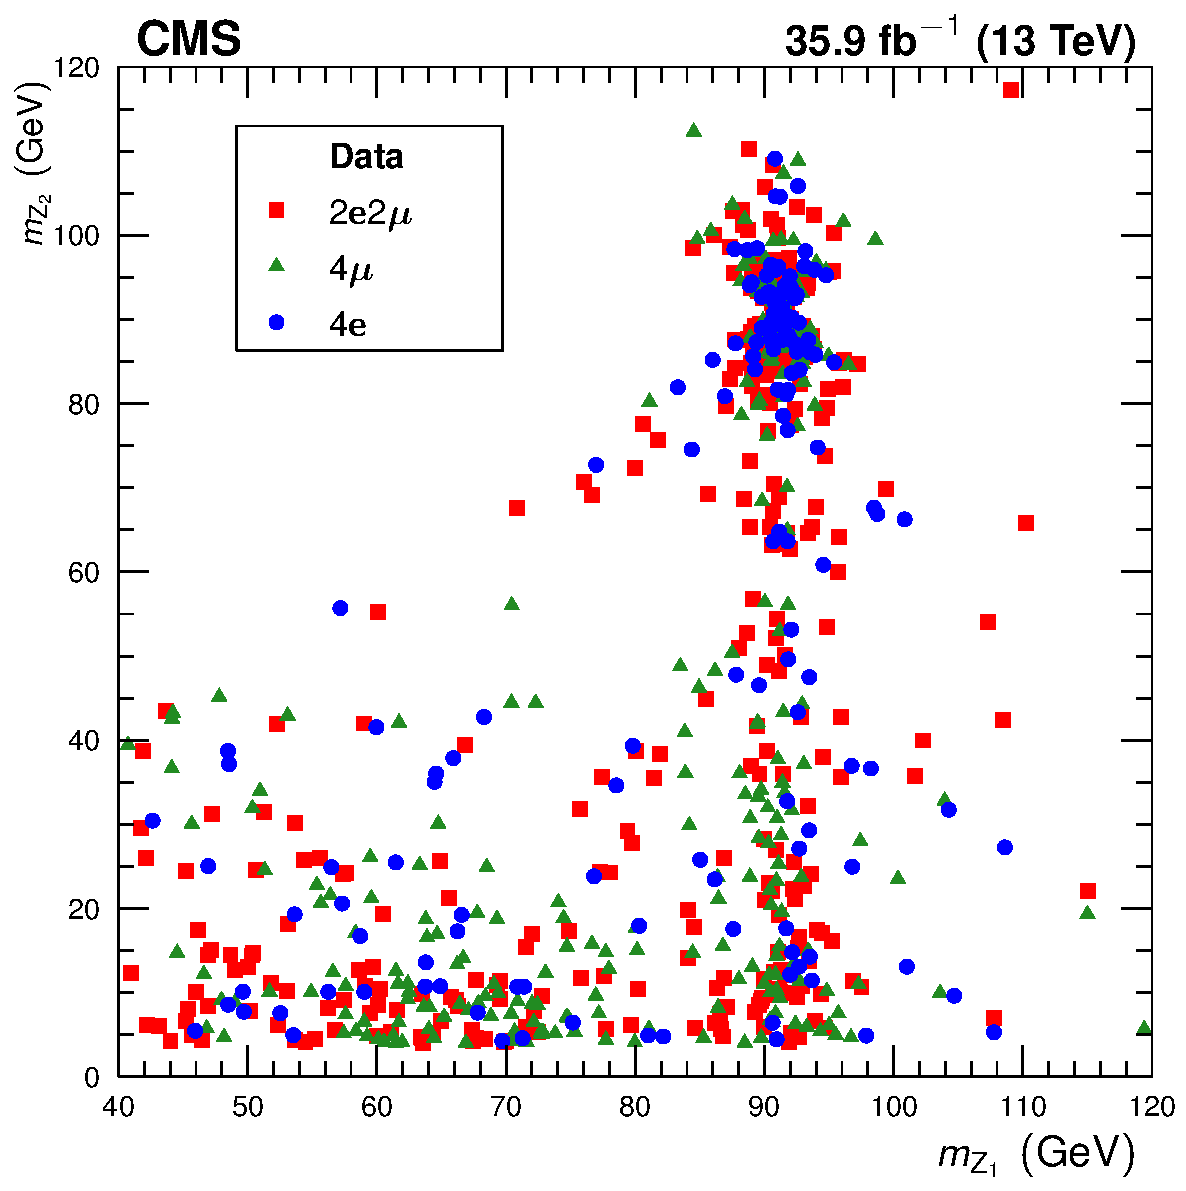
\includegraphics[width=0.75\textwidth]{results/mZ2VsmZ1_full.pdf}
    \caption[Scatter plot of $m_{\PZ_2}$ vs.\ $m_{\PZ_1}$ for data events in the full spectrum selection]{
        The reconstructed $m_{\PZ_2}$ mass plotted against the reconstructed $m_{\PZ_1}$ for data events in the full spectrum selection, with distinctive markers for each final state.
        For readability, only every fourth event is drawn.
      }\label{fig:mZ2VsmZ1_full}
  \end{center}
\end{figure}


\subsection[\texorpdfstring{$\mathrm{Z} \to 4\ell$}{Z to 4l} Resonance]{$\mathbf{Z} \to \mathbf{4\ell}$ Resonance}

Expected and observed yields for events satisfying the {\Zfourl} selection criteria ($80 < m_{4\ell} < 100\GeV$) are shown in Table~\ref{tab:results_z4l}.
The invariant mass distribution of these events is shown in Fig.~\ref{fig:mass_z4l}.
Figure~\ref{fig:mZ2VsmZ1_z4l} shows $m_{\PZ_2}$ plotted against $m_{\PZ_1}$ for all data events consistent with {\Zfourl} production.
Predictions from Monte Carlo samples generally agree well with the data.

\begin{table}[htbp]
  \begin{center}
    \caption[Expected and observed yields for {\Zfourl} production.]{
      Observed and expected yields of {\Zfourl} events, including expected background yields, shown for each final state and summed to the total.
      Uncertainties are statistical, then systematic, not including the integrated luminosity uncertainty.
    }\label{tab:results_z4l}
    \begin{tabular}{ccccc}
      \toprule
      Final & Expected     &  Background   & Total     & Observed \\
      state & $N_{4\ell}$  &               & expected  &          \\
      \midrule
      \midrule
      $4\Pm$       & $ 224 \pm 1 \pm 16   $  & $ 7 \pm 1 \pm 2    $  & $ 231 \pm 2 \pm 17   $  & $ 225 $  \\
      $2\Pe 2\Pm$  & $ 207 \pm 1 \pm 14   $  & $ 9 \pm 1 \pm 2    $  & $ 216 \pm 2 \pm 14   $  & $ 206 $  \\
      $4\Pe$       & $ 68 \pm 1 \pm 8     $  & $ 4 \pm 1 \pm 2    $  & $ 72 \pm 1 \pm 8     $  & $ 78  $  \\
      \midrule
      Total        & $ 499  \pm 2  \pm 32 $  & $ 19  \pm 2  \pm 5 $  & $ 518  \pm 3  \pm 33 $  & $ 509 $  \\
      \bottomrule
    \end{tabular}
  \end{center}
\end{table}

\begin{figure}[htbp]
  \begin{center}
    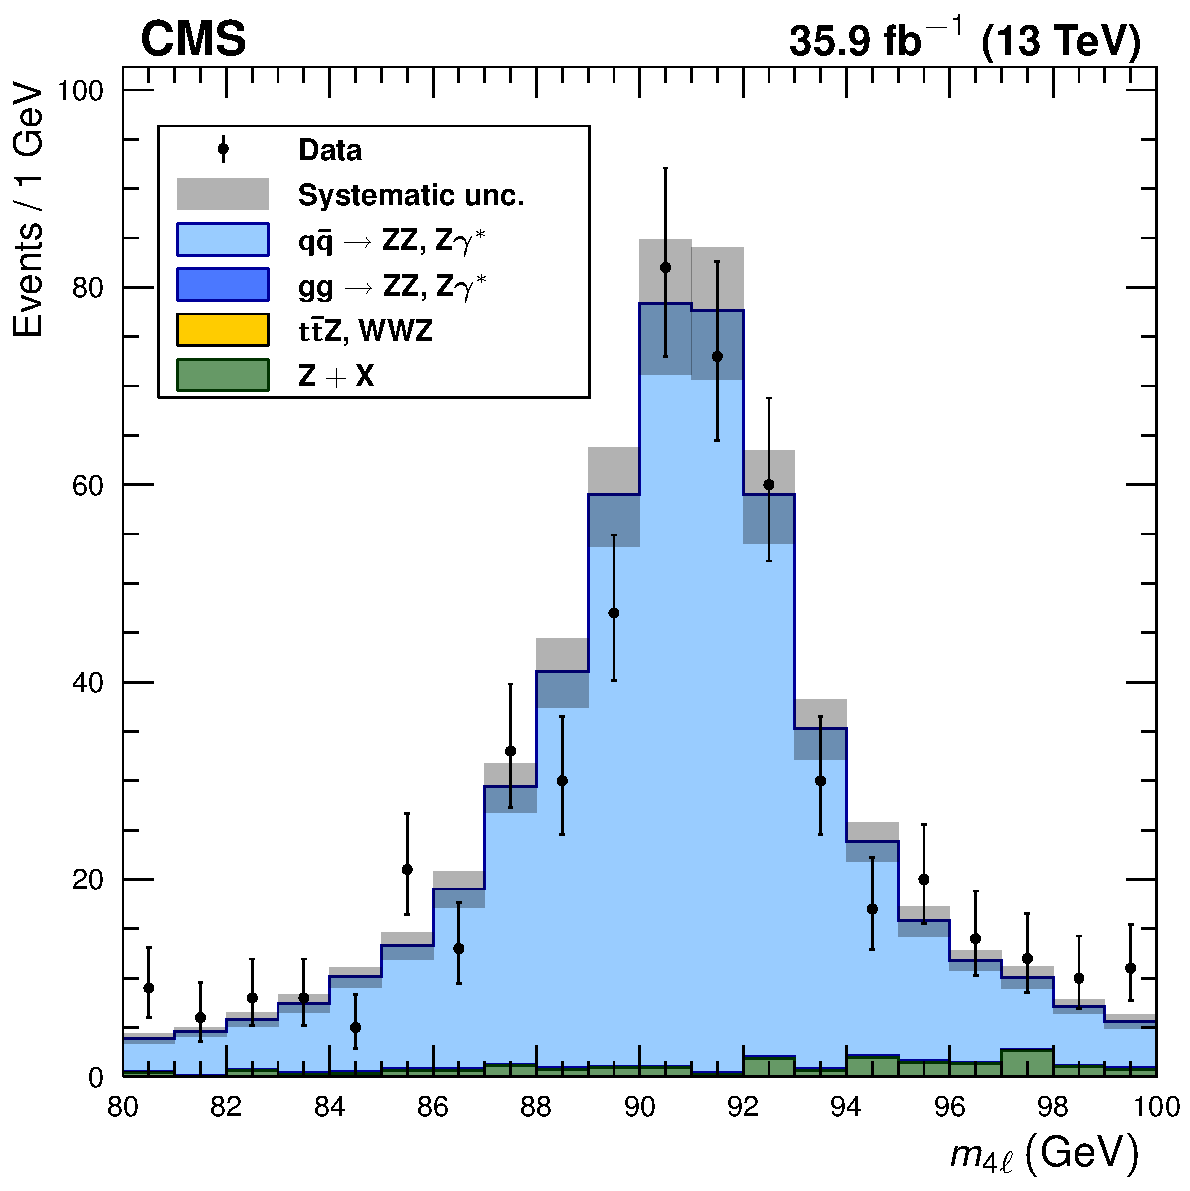
\includegraphics[width=0.75\textwidth]{results/z4lzzMass.pdf}
    \caption[Four-lepton mass in the {\Zfourl} selection]{
        Distribution of the four-lepton invariant mass $m_{4\ell}$ of all events in the mass range $80 < m_{4\ell} < 100\GeV$, the {\Zfourl} selection.
        Points represent data, with statistical uncertainty bars.
        The stack of filled histograms represents the SM signal prediction and background estimate, with a grey band showing the sum in quadrature of the statistical and systematic uncertainties on the total expected yield.
      }\label{fig:mass_z4l}
  \end{center}
\end{figure}

\begin{figure}[htbp]
  \begin{center}
    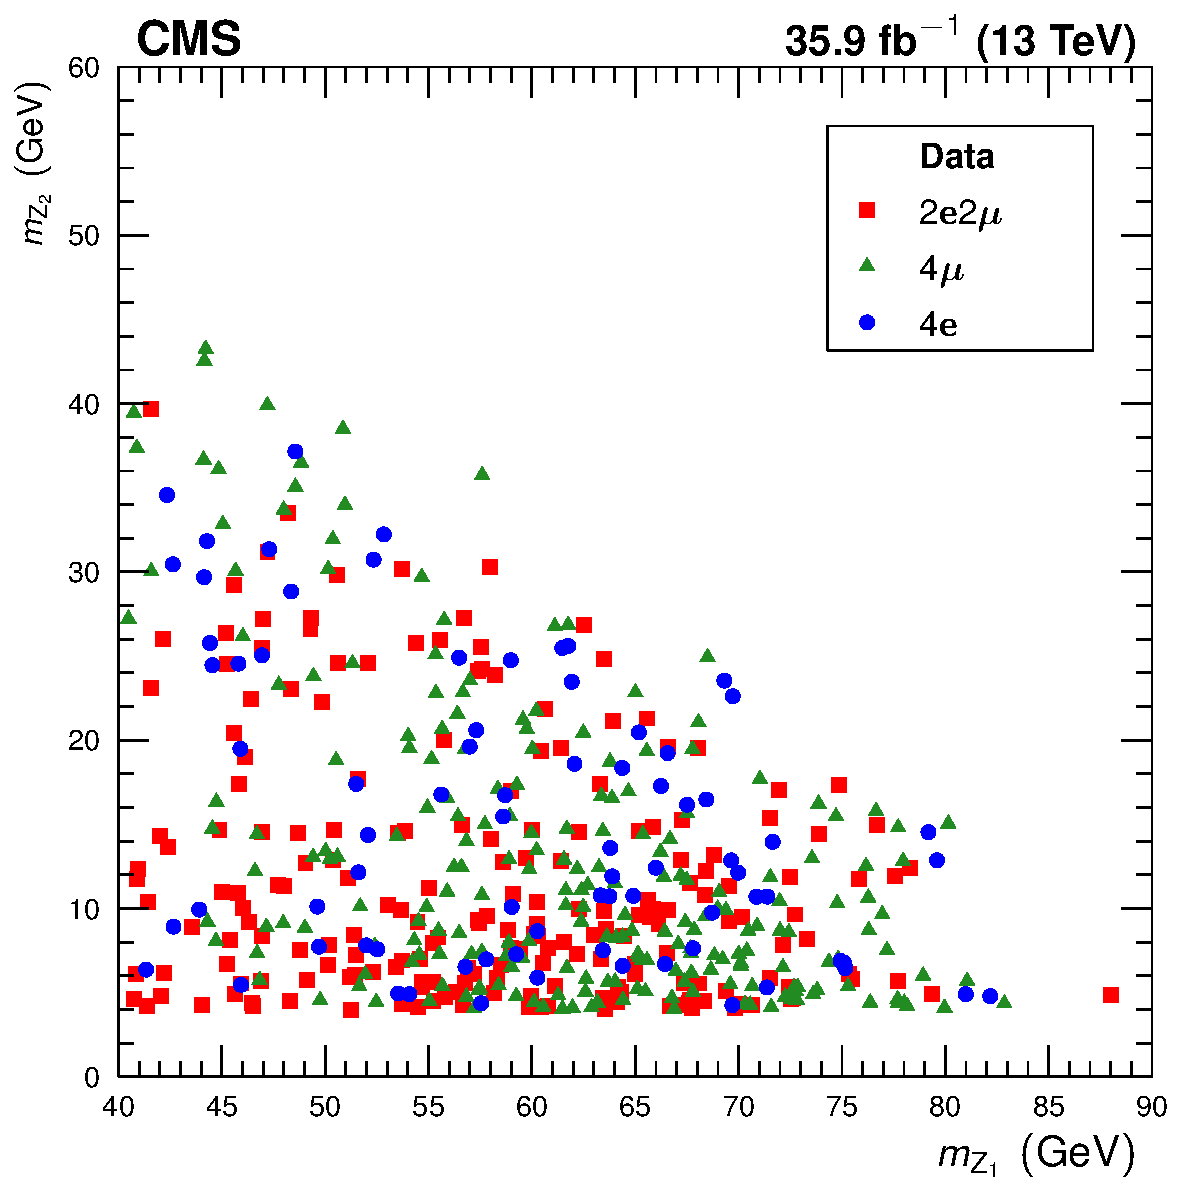
\includegraphics[width=0.75\textwidth]{results/mZ2VsmZ1_z4l.pdf}
    \caption[Scatter plot of $m_{\PZ_2}$ vs.\ $m_{\PZ_1}$ for data events in the {\Zfourl} selection]{
        The reconstructed $m_{\PZ_2}$ mass plotted against the reconstructed $m_{\PZ_1}$ for data events with $80 < m_{4\ell} < 100\GeV$, with distinctive markers for each final state.
      }\label{fig:mZ2VsmZ1_z4l}
  \end{center}
\end{figure}


\subsection{Higgs Resonance}

Figure~\ref{fig:mass_hzz} shows the four-lepton invariant mass around the Higgs resonance, which can be clearly seen above the SM continuum background, for events passing the Higgs selection ($m_{\PZ_2} > 12\GeV$, $\text{SIP}_\text{3D} < 4$ for all leptons).
Table~\ref{tab:results_hzz} shows the observed and expected yields in the mass range $118 < m_{4\ell} < 130\GeV$.
Here, SM continuum production---considered signal in all other parts of this analysis---is considered background.
Figures~\ref{fig:z1Mass_hzz}--\ref{fig:mZ2VsmZ1_hzz} show the $\PZ_1$ mass, the $\PZ_2$ mass, and the scatter plot of $m_{\PZ_2}$ against $m_{\PZ_1}$, in the same four-lepton mass region around the Higgs resonance.
Agreement between predictions and data is again good.

\begin{table}[htbp]
  \begin{center}
    \caption[Expected and observed yields for Higgs boson production.]{
      Observed and expected yields of $\PH \to \PZ\PZ^\ast \to 4\ell$ events, including expected background yields, for events passing the Higgs selection in the mass range $118 < m_{4\ell} < 130\GeV$, shown for each final state and summed to the total.
      Uncertainties are statistical and systematic combined.
    }\label{tab:results_hzz}
    \begin{tabular}{cccccc}
      \toprule
      Final & Expected   &  SM continuum & $\PZ + \PX$  & Total     & Observed \\
      state & $N_\PH$    &  background   &              & expected  &          \\
      \midrule
      \midrule
      $4\Pm$       & $ 21.6 \pm 1.9   $  & $ 9.4  ^{+0.6}_{-0.7}   $  & $ 4.7  ^{+2.0}_{-1.8}  $  & $ 35.8 \pm 2.9        $  & $ 34 $ \\
      $2\Pe 2\Pm$  & $ 26.5 \pm 2.3   $  & $ 11.0 ^{+0.7}_{-0.8}   $  & $ 6.9  ^{+3.1}_{-2.9}  $  & $ 44.4 ^{+3.7}_{-3.6} $  & $ 41 $ \\
      $4\Pe$       & $ 10.2 \pm 1.1   $  & $ 3.6  \pm 0.3          $  & $ 1.9  ^{+0.8}_{-1.0}  $  & $ 15.8 \pm 1.6        $  & $ 19 $ \\
      \midrule
      Total        & $ 58.3 \pm 5.0   $  & $ 24.1 ^{+1.5}_{-1.6}   $  & $ 13.5 ^{+3.7}_{-3.5}  $  & $ 96.0 \pm 6.7        $  & $ 94 $ \\
      \bottomrule
    \end{tabular}
  \end{center}
\end{table}

\begin{figure}[htbp]
  \begin{center}
    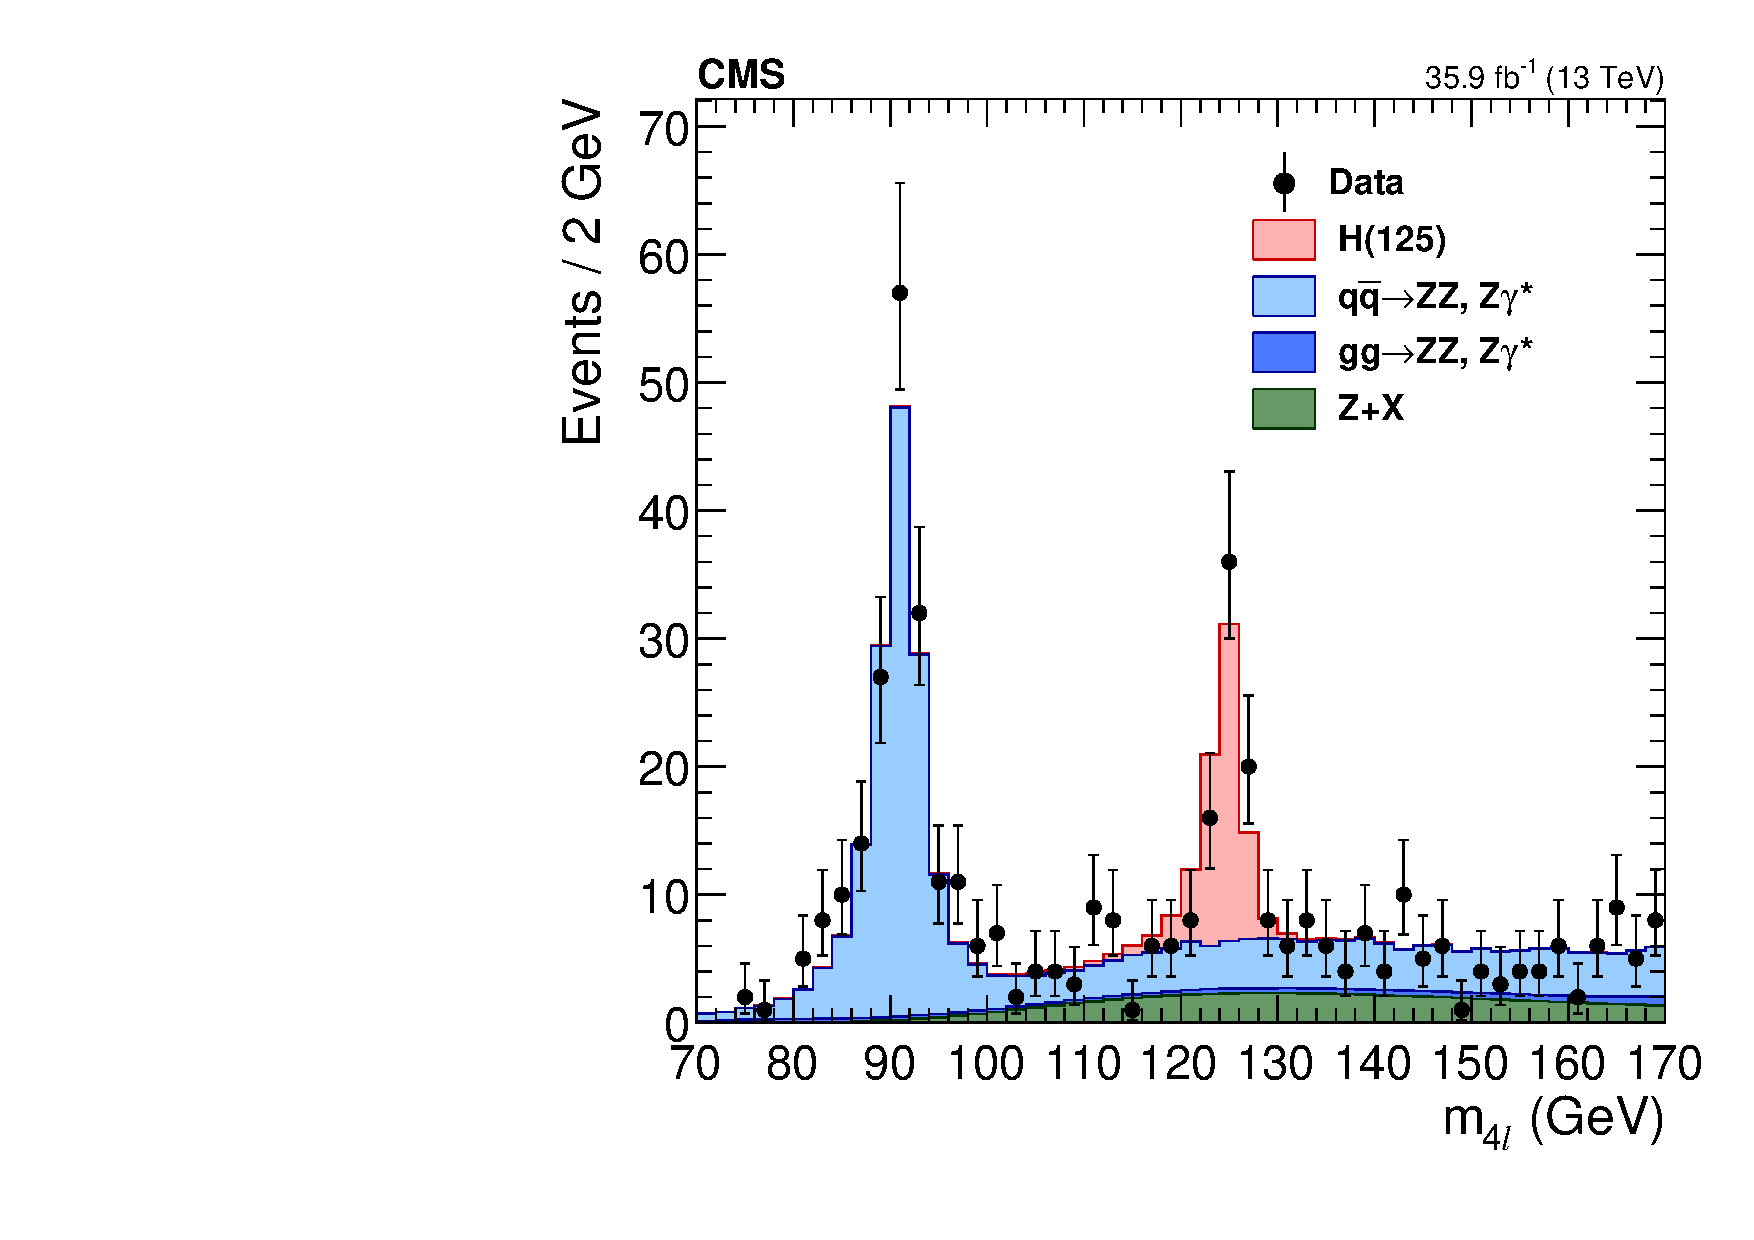
\includegraphics[width=0.75\textwidth]{results/hzzMass.pdf}
    \caption[Four-lepton mass spectrum around the Higgs resonance]{
        Distribution of the four-lepton invariant mass $m_{4\ell}$ of events in the Higgs selection.
        Points represent data, with statistical uncertainty bars.
        The stack of filled histograms represents the SM signal prediction and background estimate.
      }\label{fig:mass_hzz}
  \end{center}
\end{figure}

\begin{figure}[htbp]
  \begin{center}
    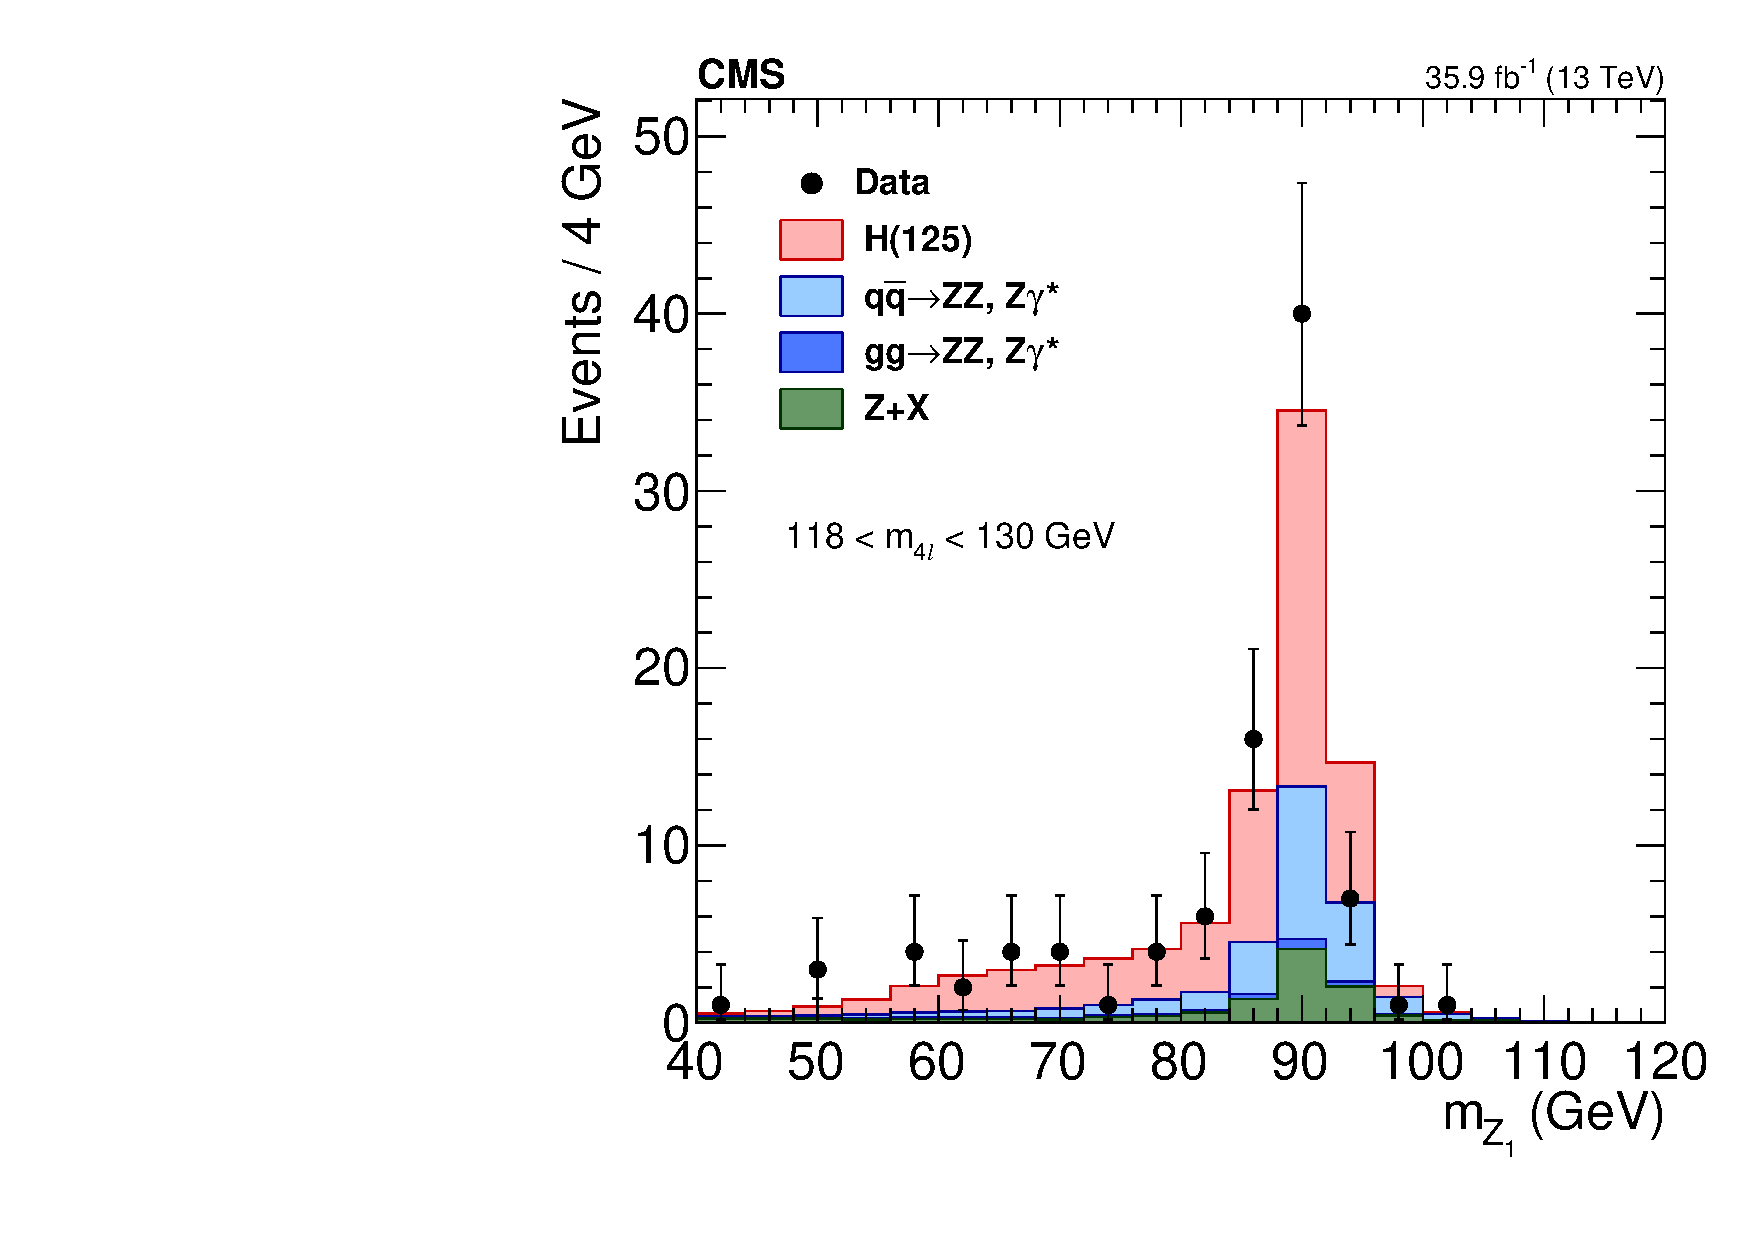
\includegraphics[width=0.75\textwidth]{results/hzzz1Mass.pdf}
    \caption[Mass of $\PZ_1$ candidates in events near the Higgs resonance]{
        Distribution of the dilepton invariant mass of $\PZ_1$, the dilepton candidate in each event closest to the nominal $m_\PZ$, in events in the Higgs selection with $118 < m_{4\ell} < 130\GeV$.
        Points represent data, with statistical uncertainty bars.
        The stack of filled histograms represents the SM signal prediction and background estimate.
      }\label{fig:z1Mass_hzz}
  \end{center}
\end{figure}

\begin{figure}[htbp]
  \begin{center}
    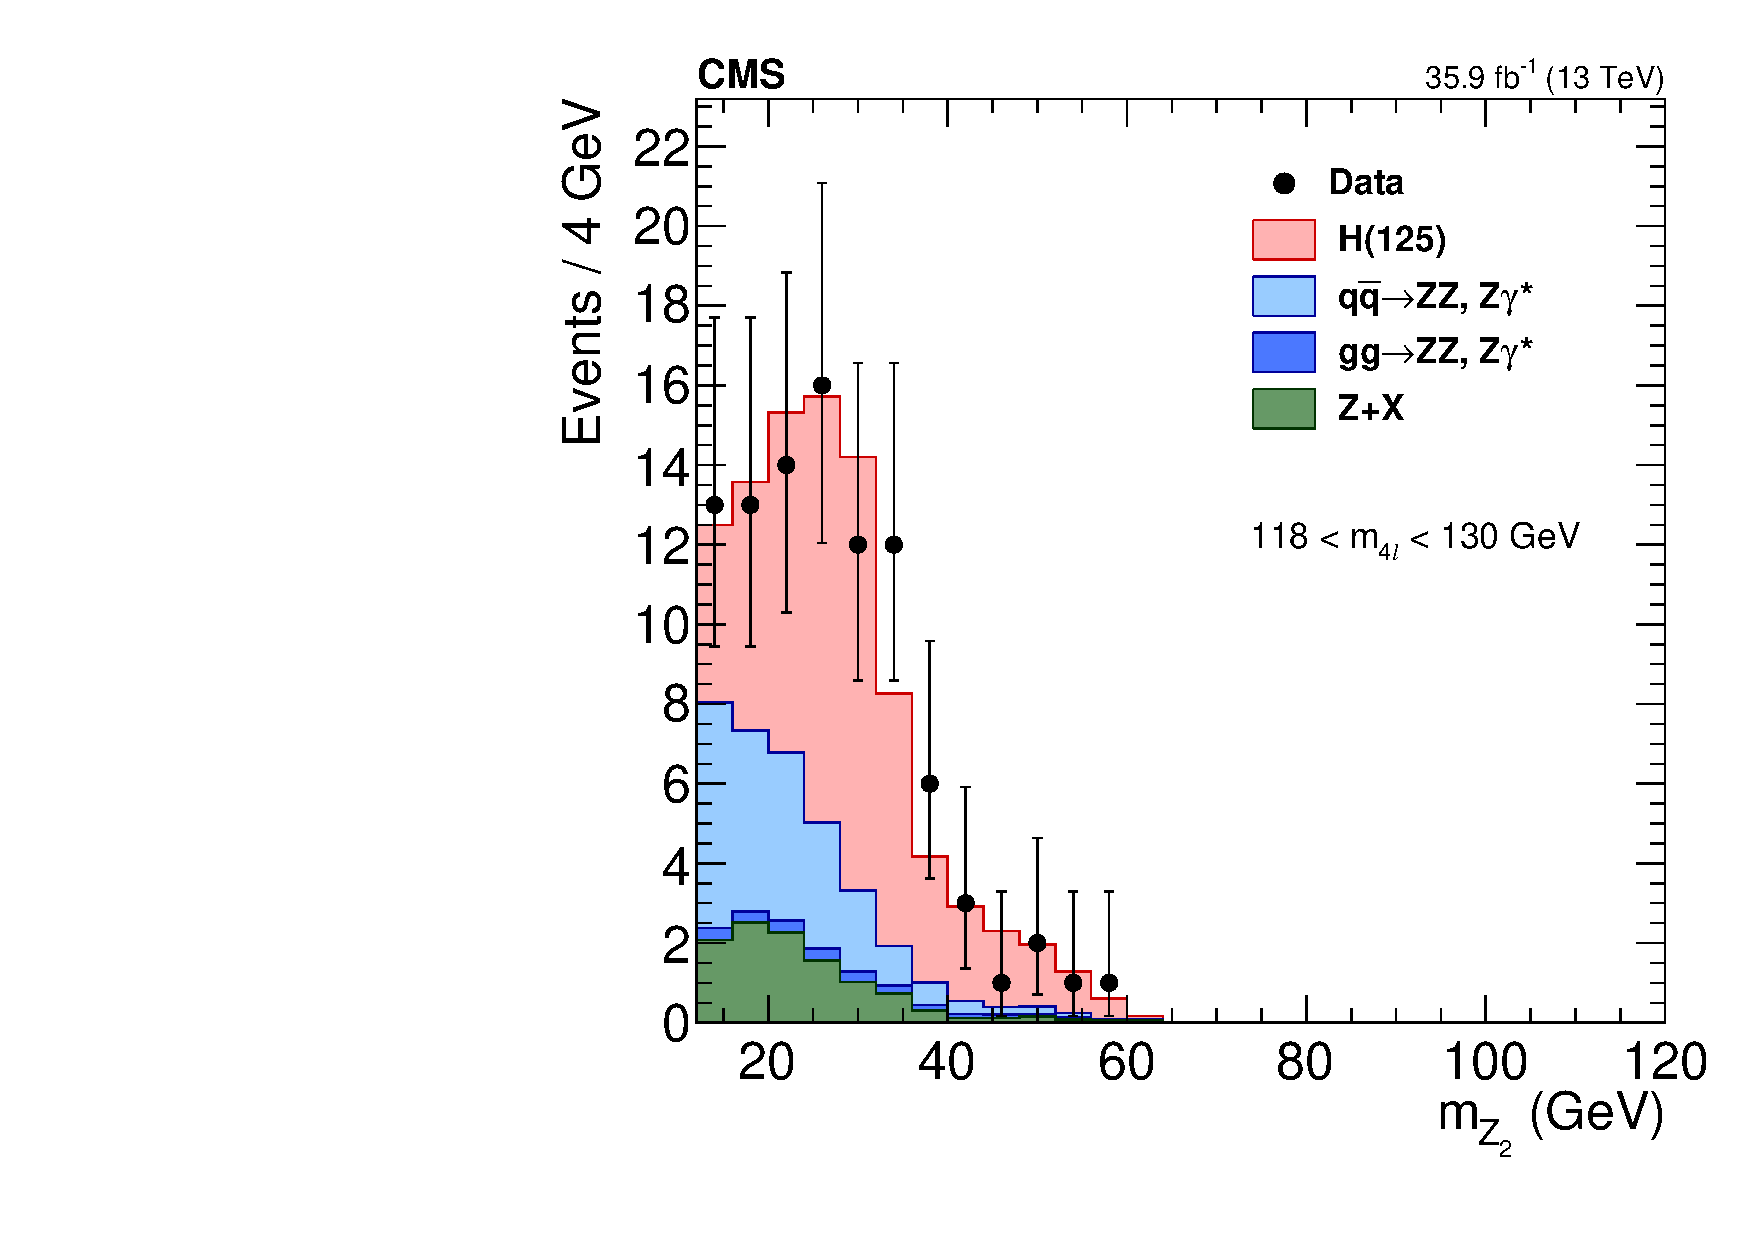
\includegraphics[width=0.75\textwidth]{results/hzzz2Mass.pdf}
    \caption[Mass of $\PZ_2$ candidates in events near the Higgs resonance]{
        Distribution of the dilepton invariant mass of $\PZ_2$, the dilepton candidate in each event farther from the nominal $m_\PZ$, in events in the Higgs selection with $118 < m_{4\ell} < 130\GeV$.
        Points represent data, with statistical uncertainty bars.
        The stack of filled histograms represents the SM signal prediction and background estimate.
      }\label{fig:z2Mass_hzz}
  \end{center}
\end{figure}

\begin{figure}[htbp]
  \begin{center}
    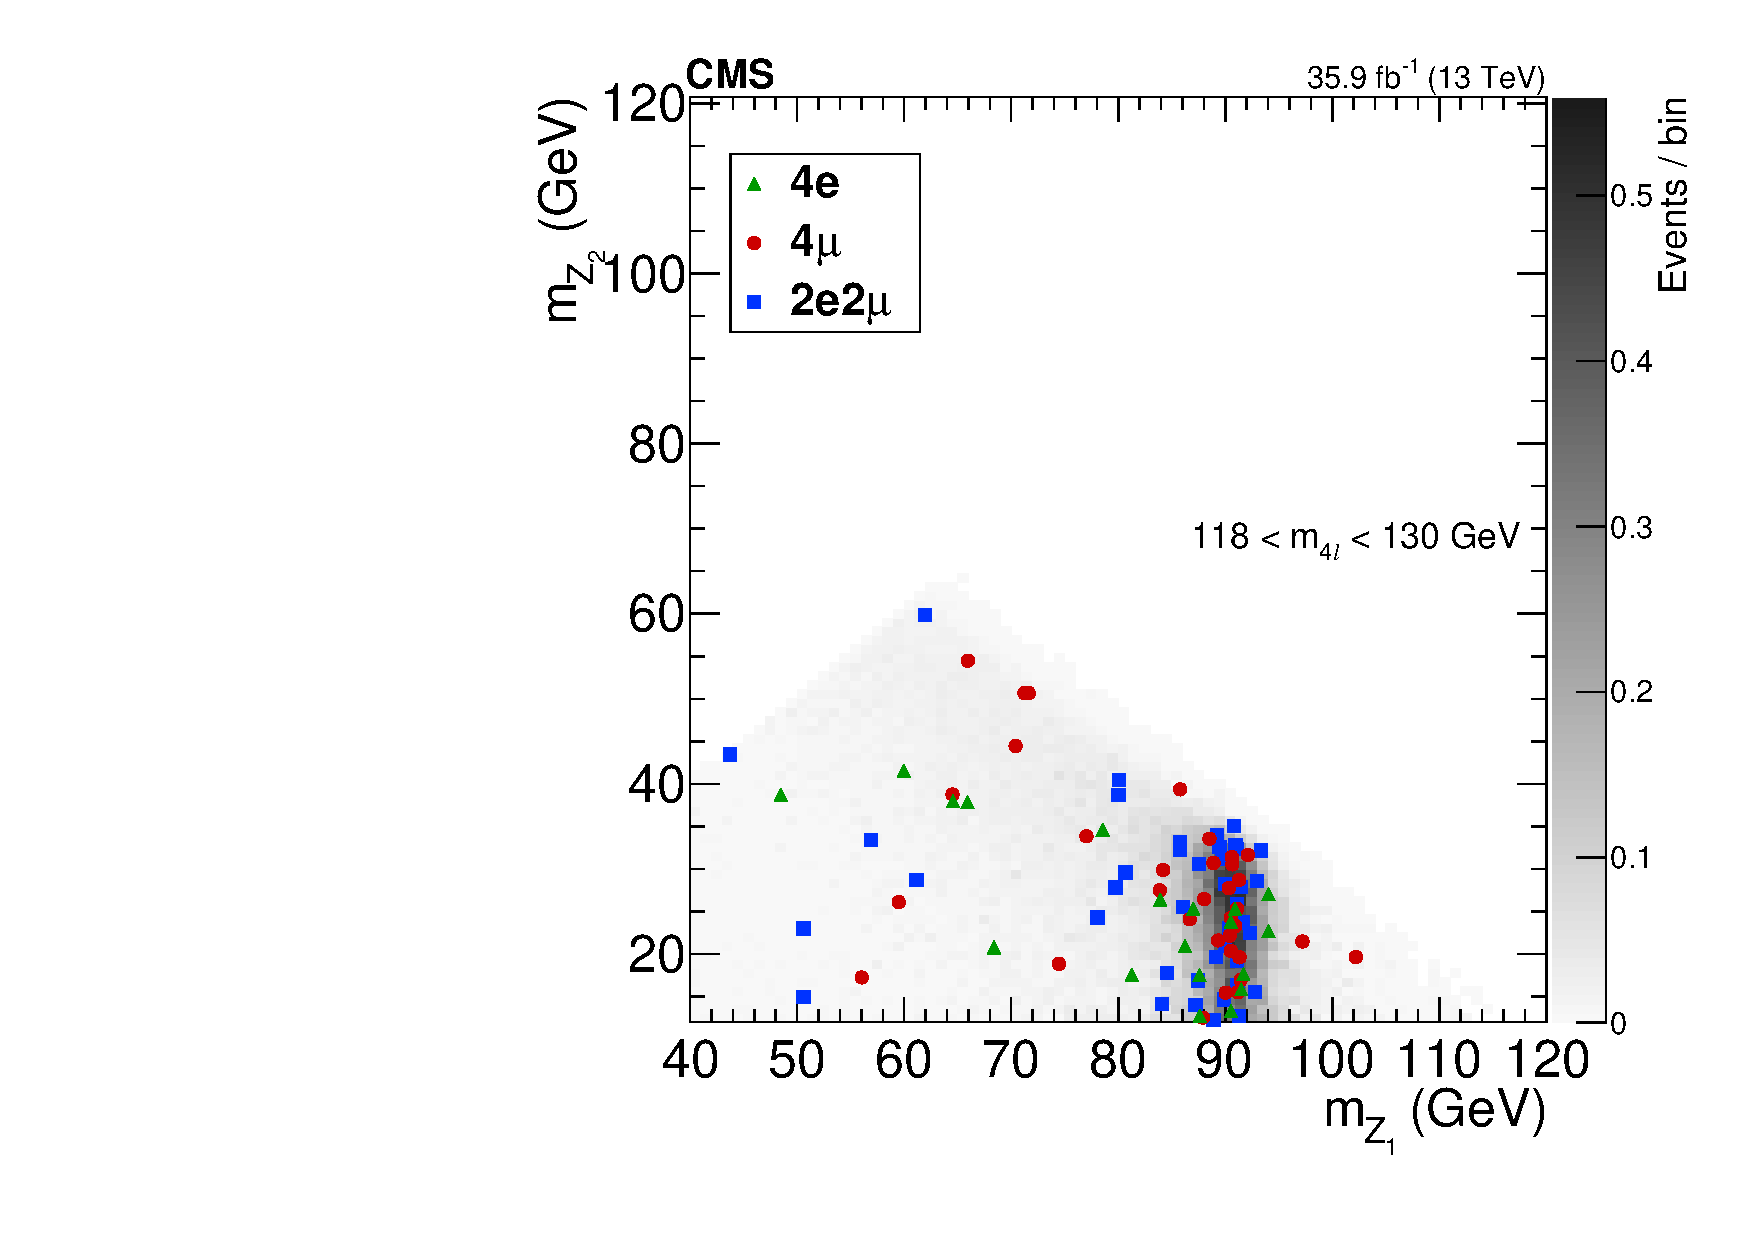
\includegraphics[width=0.75\textwidth]{results/mZ2VsmZ1_hzz.pdf}
    \caption[Scatter plot of $m_{\PZ_2}$ vs.\ $m_{\PZ_1}$ for data events near the Higgs resonance]{
        The reconstructed $m_{\PZ_2}$ mass plotted against the reconstructed $m_{\PZ_1}$ for data events in the Higgs selection with $118 < m_{4\ell} < 130\GeV$, with distinctive markers for each final state.
        The shading represents the expected number of events in the bin.
      }\label{fig:mZ2VsmZ1_hzz}
  \end{center}
\end{figure}


\subsection{ZZ Production}

Expected and observed yields for on-shell {\ZZ} events are shown in Table~\ref{tab:results_zz}.
The corresponding four-lepton and {\PZ} boson candidate invariant masses are shown in Figs.~\ref{fig:mass_smp} and~\ref{fig:zMass_smp}, respectively.
Figure~\ref{fig:njets} shows the distribution of the number of jets in these events.
The leading and subleading jet {\pt} in {\ZZ} events are shown separately in Fig.~\ref{fig:jetPt}, and the leading and subleading jet {\abseta} are shown separately in Fig.~\ref{fig:jetEta}.
Figures~\ref{fig:mjj} and~\ref{fig:deltaEtajj} show the $m_{\Pj\Pj}$ and $\lvert \Delta \eta_{\Pj\Pj} \rvert$ distributions for tagging jet pairs in the dijet selection.
Agreement is, again, overall good.

\begin{table}[htbp]
  \begin{center}
    \caption[Expected and observed yields for doubly-resonant {\ZZ} production.]{
      Observed and expected yields of {\ZZ} events, including expected background yields, in the on-shell selection, shown for each final state and summed to the total.
      Uncertainties are statistical, then systematic, not including the integrated luminosity uncertainty.
    }\label{tab:results_zz}
    \begin{tabular}{ccccc}
      \toprule
      Final & Expected   &  Background   & Total     & Observed \\
      state & $N_{\ZZ}$  &               & expected  &          \\
      \midrule
      \midrule
      $4\Pm$       & $ 301 \pm 2 \pm 9     $  & $ 10 \pm 1 \pm 2   $  & $ 311 \pm 2 \pm 9     $  & $ 335 $   \\
      $2\Pe 2\Pm$  & $ 503 \pm 2 \pm 19    $  & $ 31 \pm 2 \pm 4   $  & $ 534 \pm 3 \pm 20    $  & $ 543 $   \\
      $4\Pe$       & $ 205 \pm 1 \pm 12    $  & $ 20 \pm 2 \pm 2   $  & $ 225 \pm 2 \pm 13    $  & $ 220 $   \\
      \midrule
      Total        & $ 1009  \pm 3  \pm 36 $  & $ 60  \pm 3  \pm 8 $  & $ 1070  \pm 4  \pm 37 $  & $ 1098 $  \\
      \bottomrule
    \end{tabular}
  \end{center}
\end{table}

\begin{figure}[htbp]
  \begin{center}
    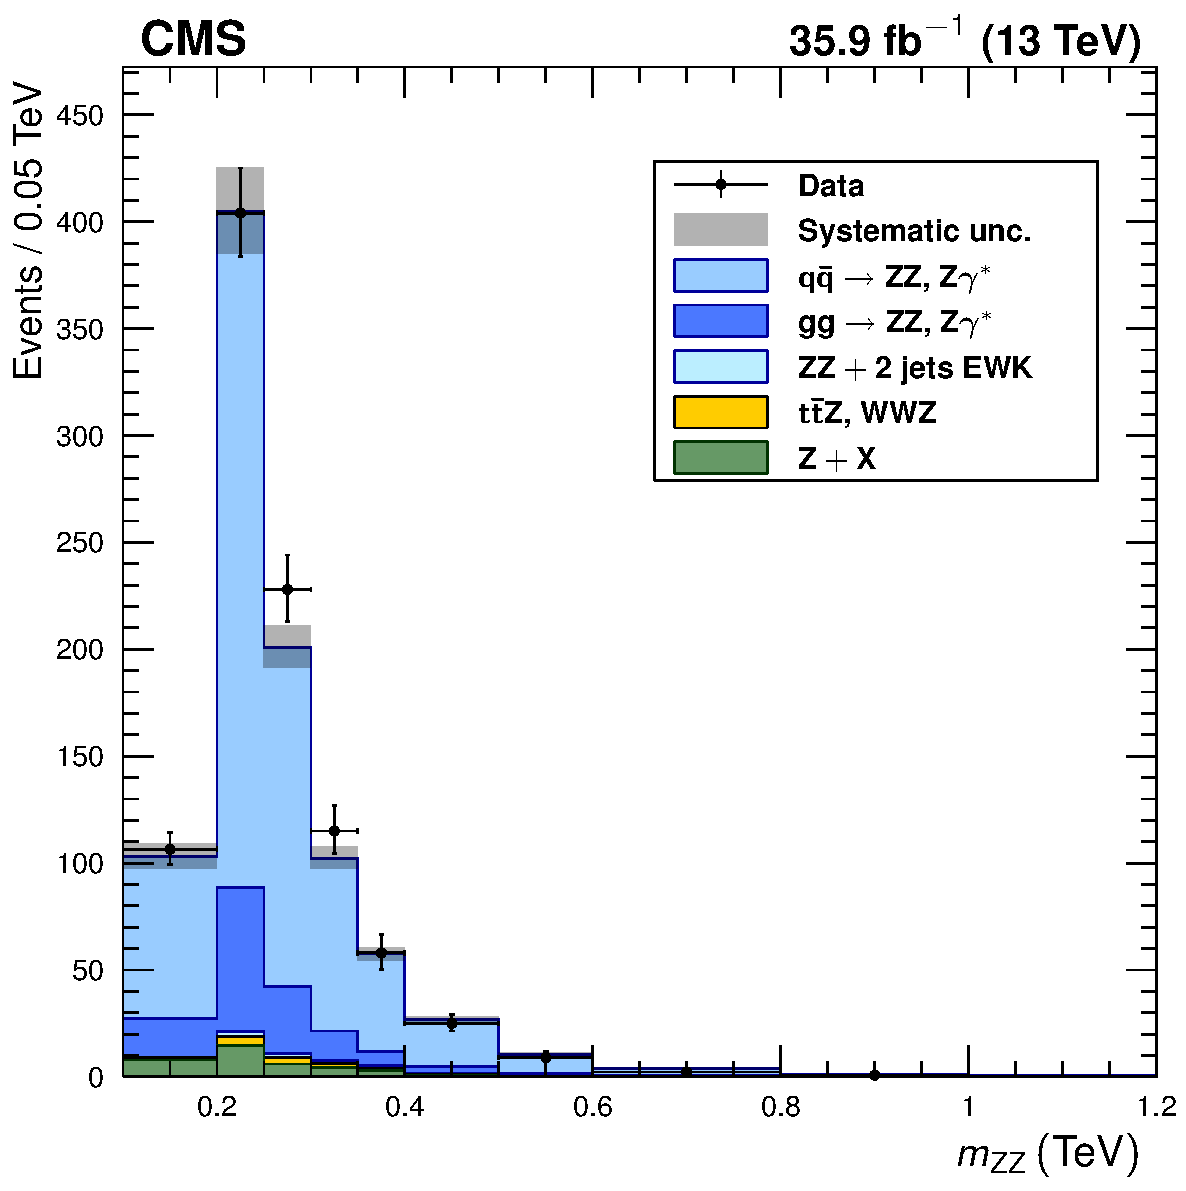
\includegraphics[width=0.75\textwidth]{results/smpzzMass.pdf}
    \caption[Four-lepton mass spectrum for events with both {\PZ} candidates on-shell]{
        Distribution of the four-lepton invariant mass $m_{\ZZ}$ of all events in the on-shell selection.
        Points represent data, with statistical uncertainty bars.
        The stack of filled histograms represents the SM signal prediction and background estimate, with a grey band showing the sum in quadrature of the statistical and systematic uncertainties on the total expected yield.
      }\label{fig:mass_smp}
  \end{center}
\end{figure}

\begin{figure}[htbp]
  \begin{center}
    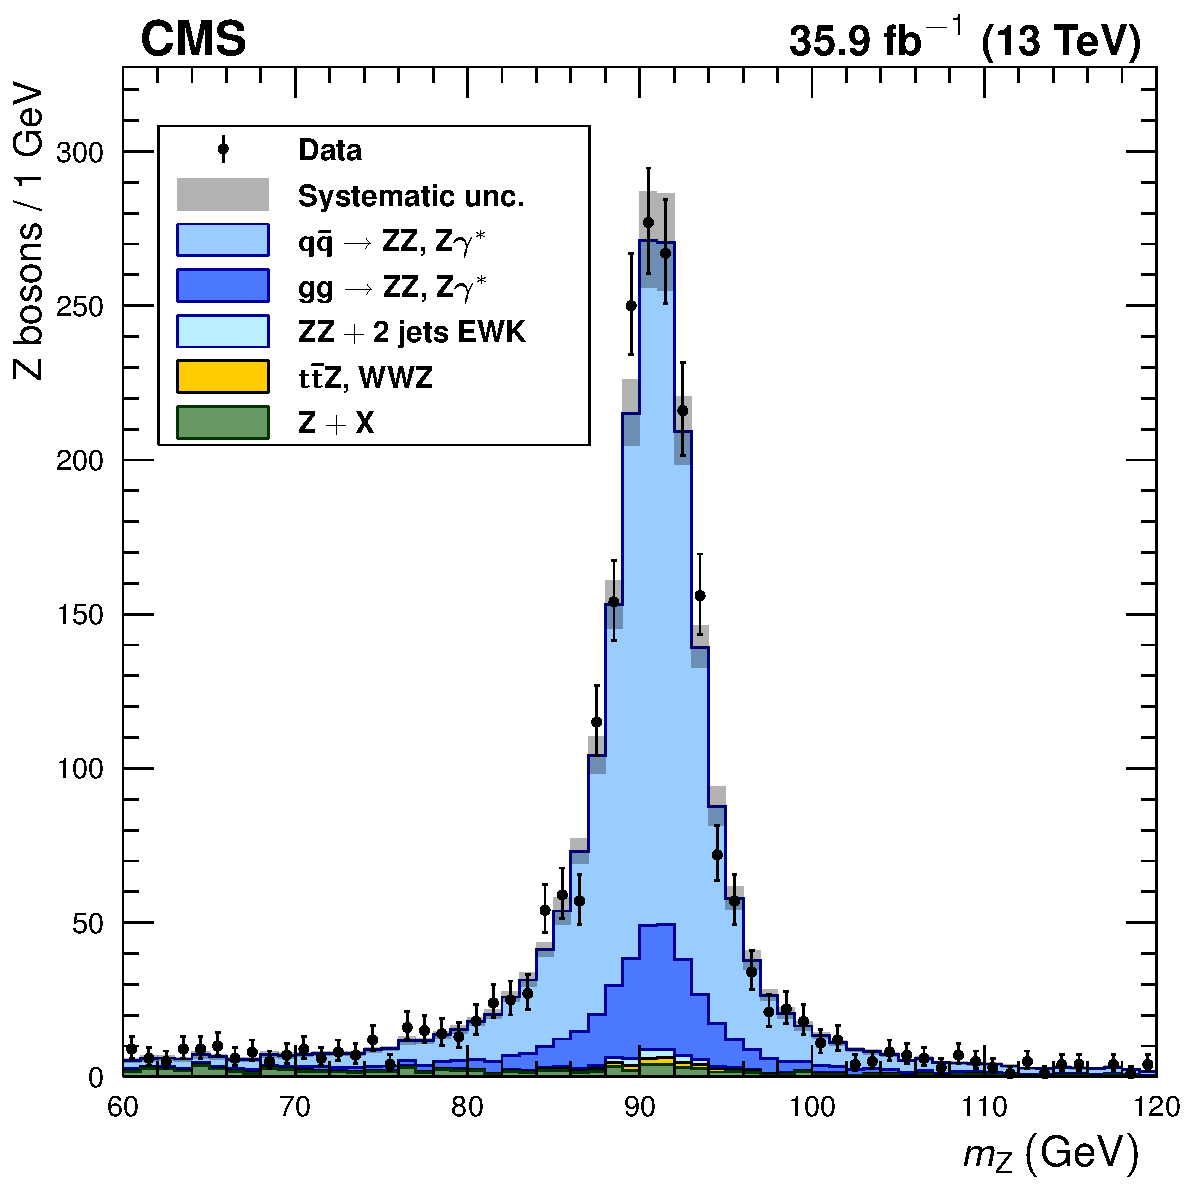
\includegraphics[width=0.75\textwidth]{results/smpzMass.pdf}
    \caption[Mass of all {\Zgs} candidates in the on-shell selection]{
        Distribution of the dilepton invariant mass of {\PZ} candidates in all events in the on-shell selection, regardless of whether the lepton pair is labeled $\PZ_1$ or $\PZ_2$.
        Points represent data, with statistical uncertainty bars.
        The stack of filled histograms represents the SM signal prediction and background estimate, with a grey band showing the sum in quadrature of the statistical and systematic uncertainties on the total expected yield.
      }\label{fig:zMass_smp}
  \end{center}
\end{figure}

\begin{figure}[htbp]
  \begin{center}
    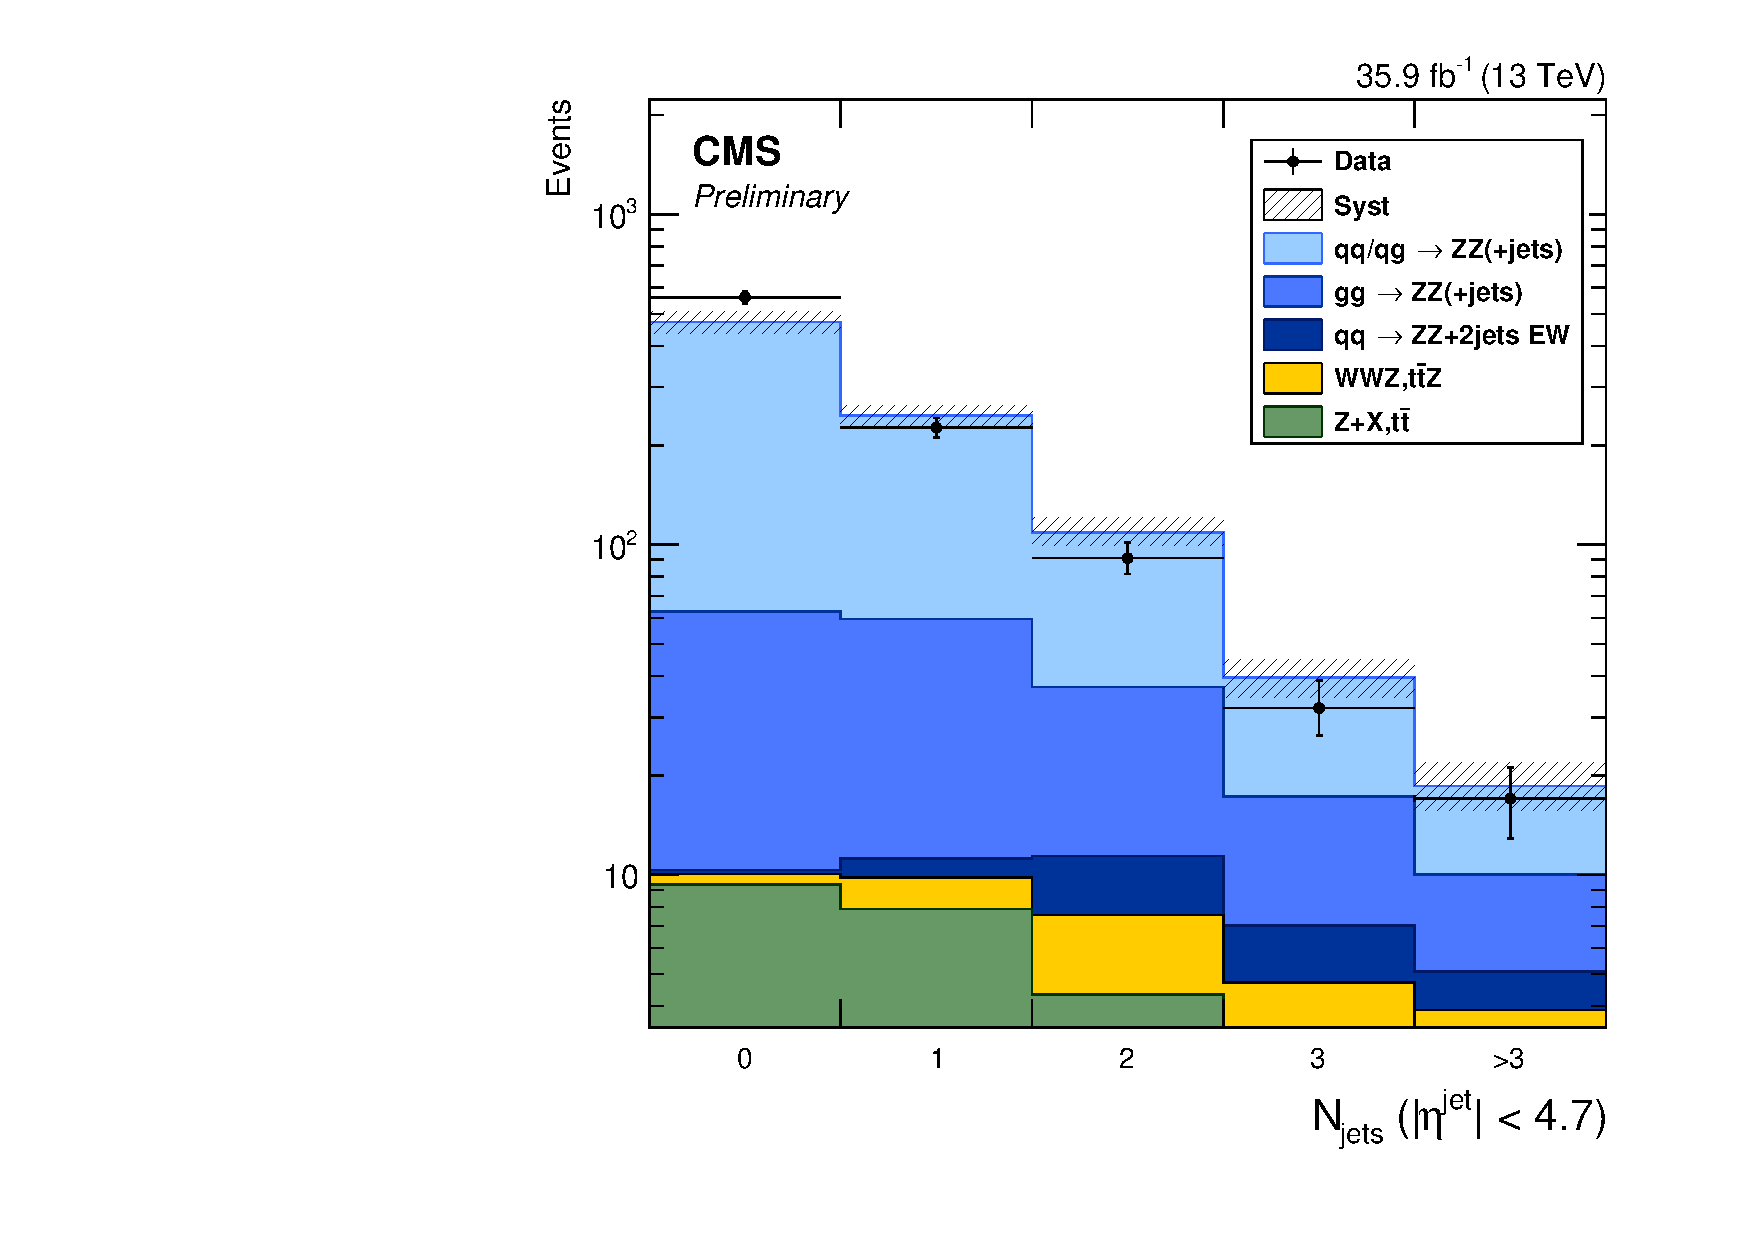
\includegraphics[width=0.75\textwidth]{results/njets.pdf}
    \caption[Jet multiplicity]{
        Distribution of jet multiplicity in {\ZZ} events.
        Points represent data, with statistical uncertainty bars.
        The stack of filled histograms represents the SM signal prediction and background estimate, with a hatched band showing the sum in quadrature of the statistical and systematic uncertainties on the total expected yield.
      }\label{fig:njets}
  \end{center}
\end{figure}

\begin{figure}[htbp]
  \begin{center}
    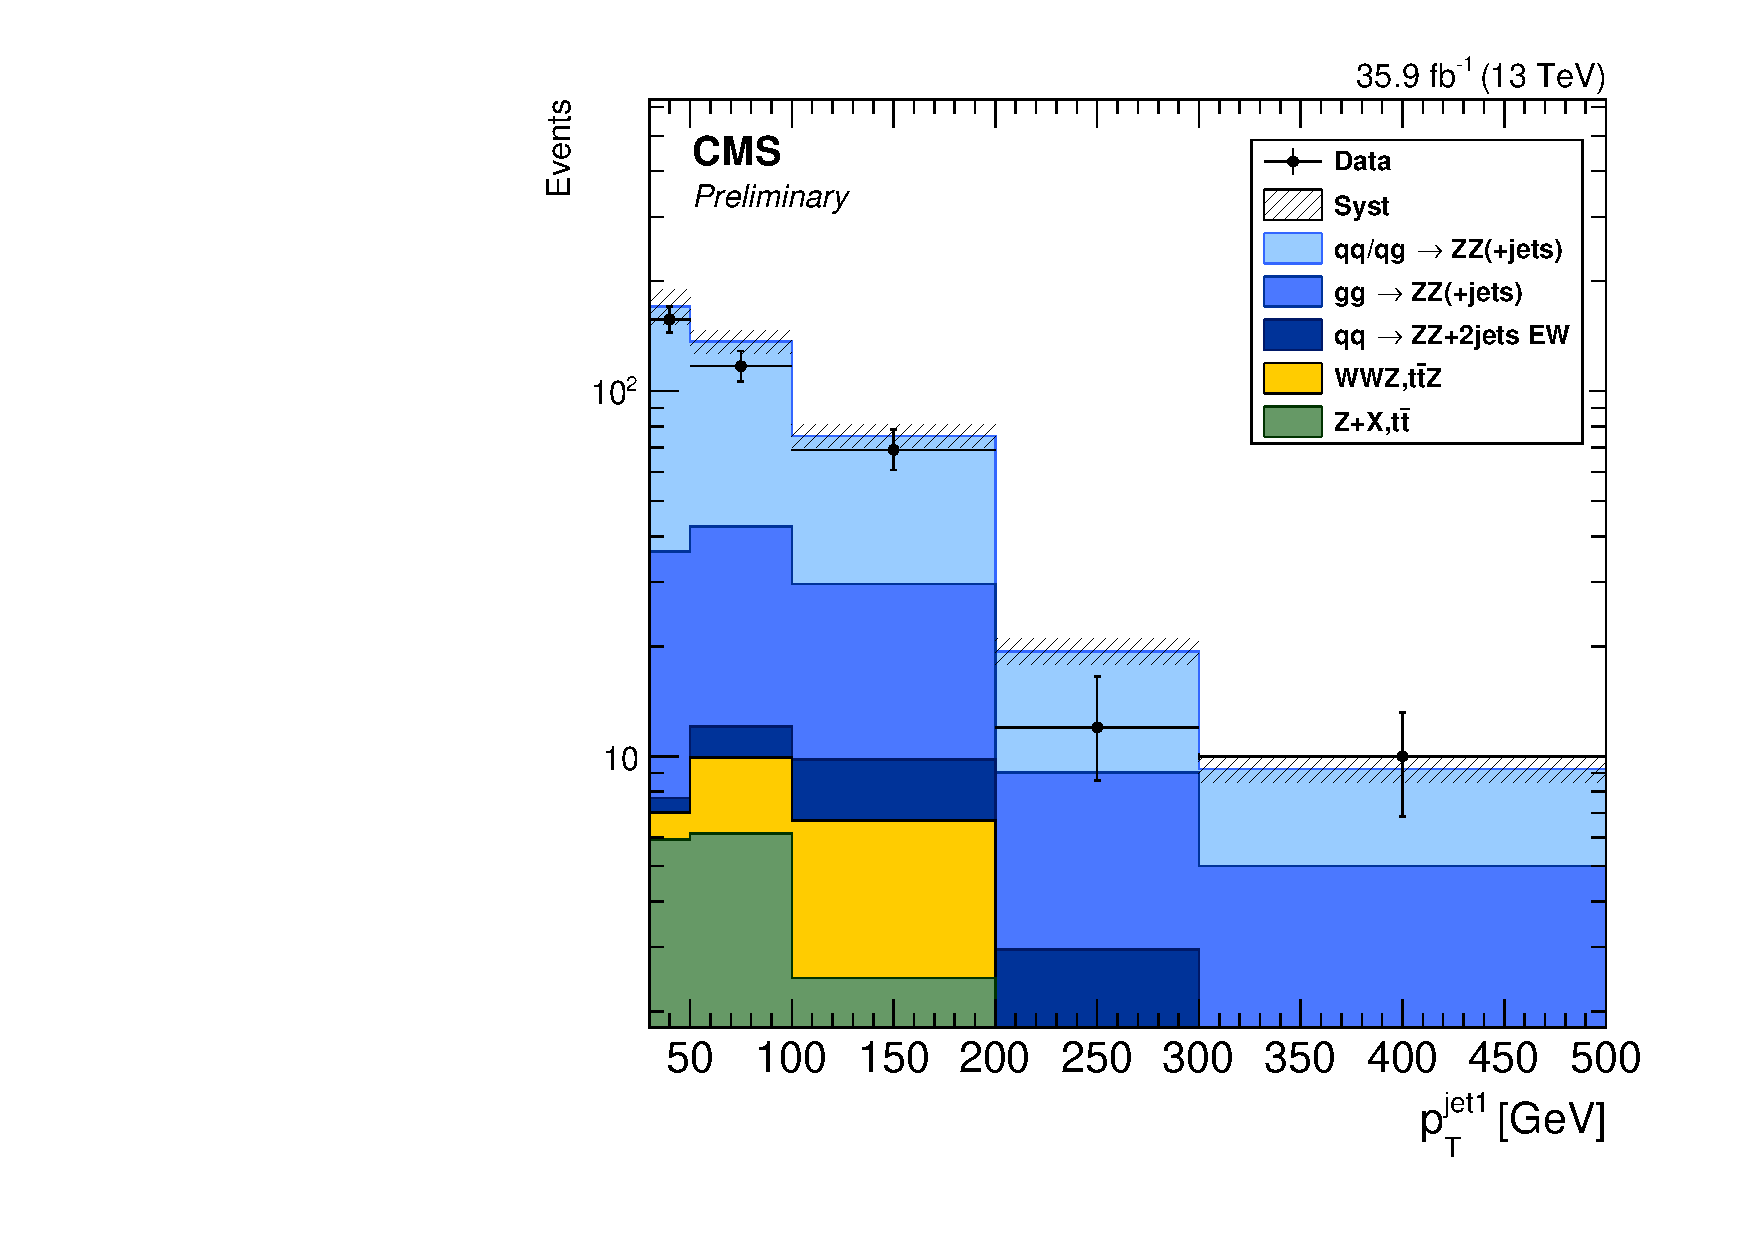
\includegraphics[width=0.48\textwidth]{results/j1Pt.pdf}
    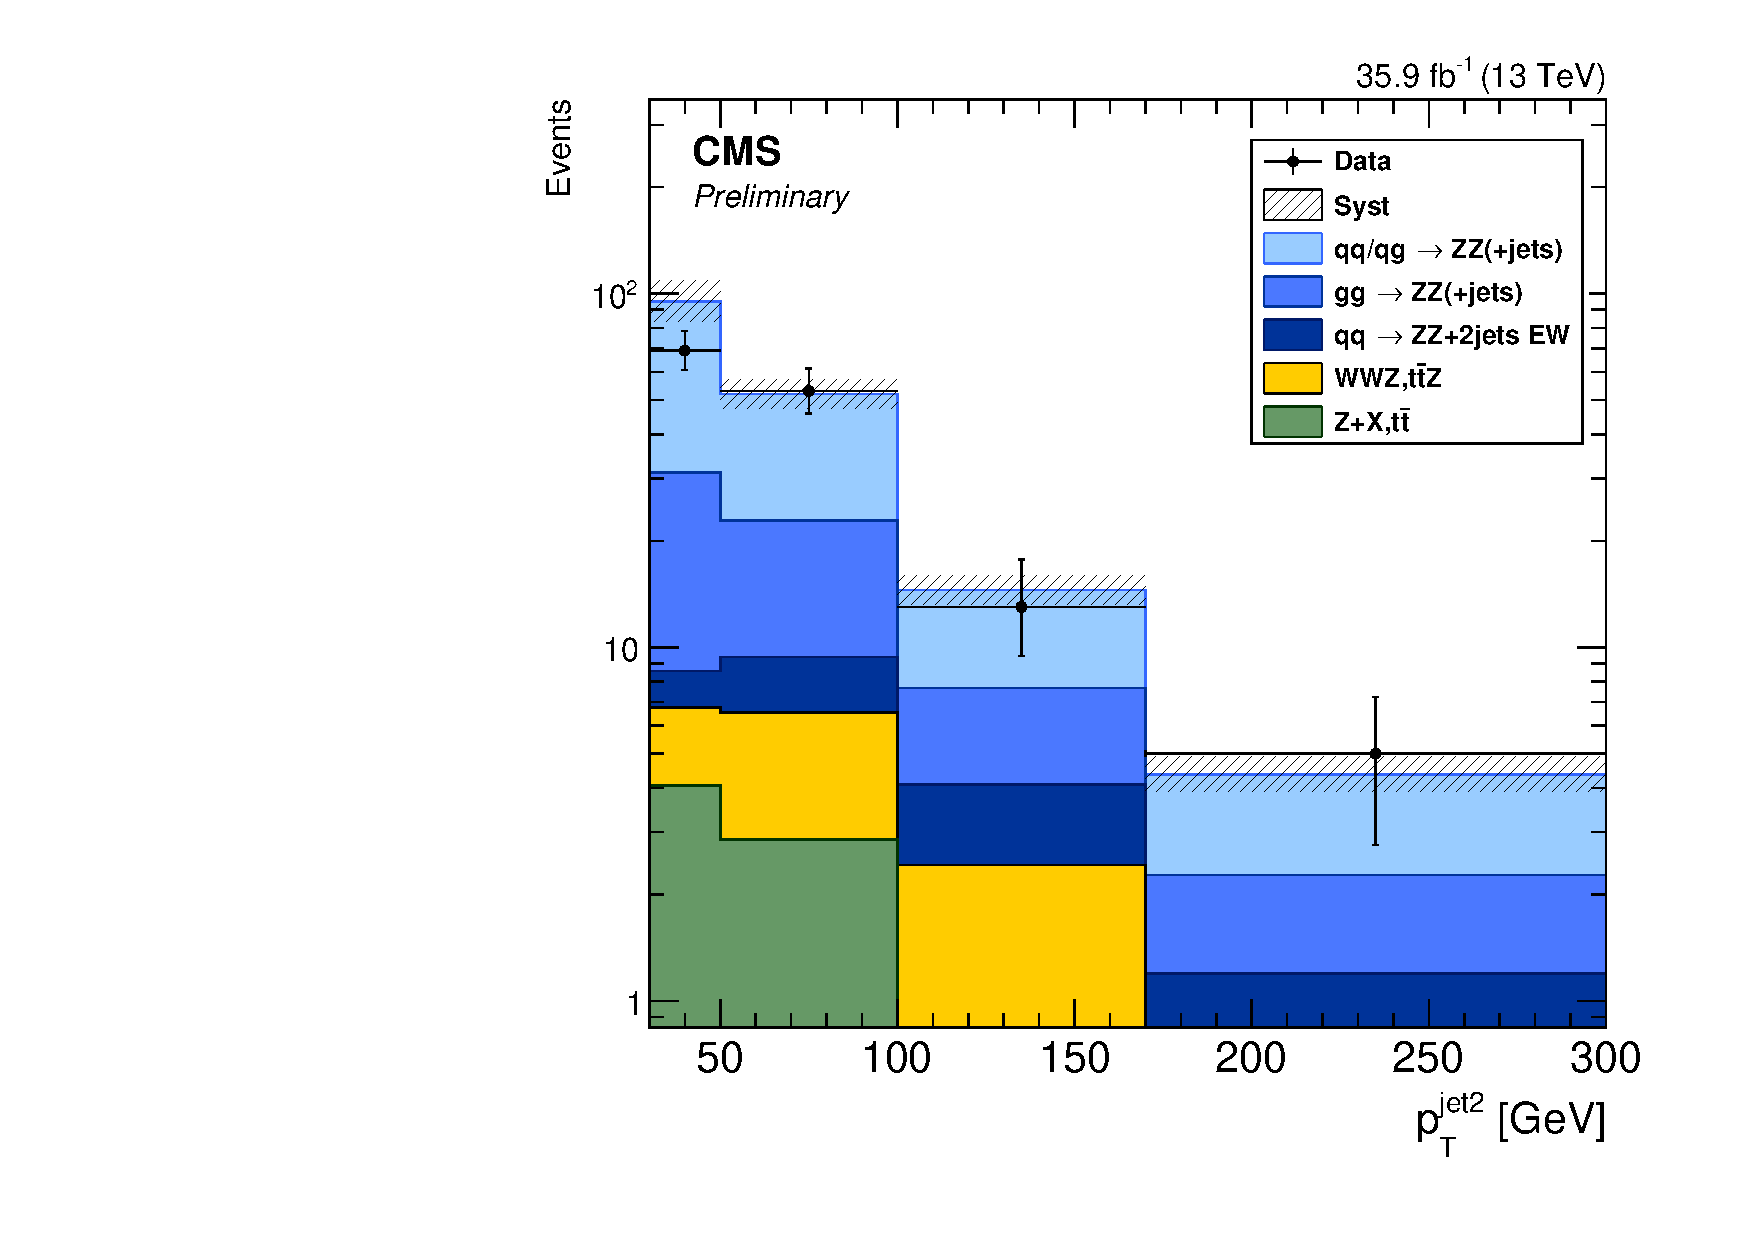
\includegraphics[width=0.48\textwidth]{results/j2Pt.pdf}
    \caption[Transverse momentum of the leading and subleading jets]{
        Distribution of leading (left) and subleading (right) jet {\pt} in {\ZZ} events with at least one jet and at least two jets, respectively.
        Points represent data, with statistical uncertainty bars.
        The stack of filled histograms represents the SM signal prediction and background estimate, with a hatched band showing the sum in quadrature of the statistical and systematic uncertainties on the total expected yield.
      }\label{fig:jetPt}
  \end{center}
\end{figure}

\begin{figure}[htbp]
  \begin{center}
    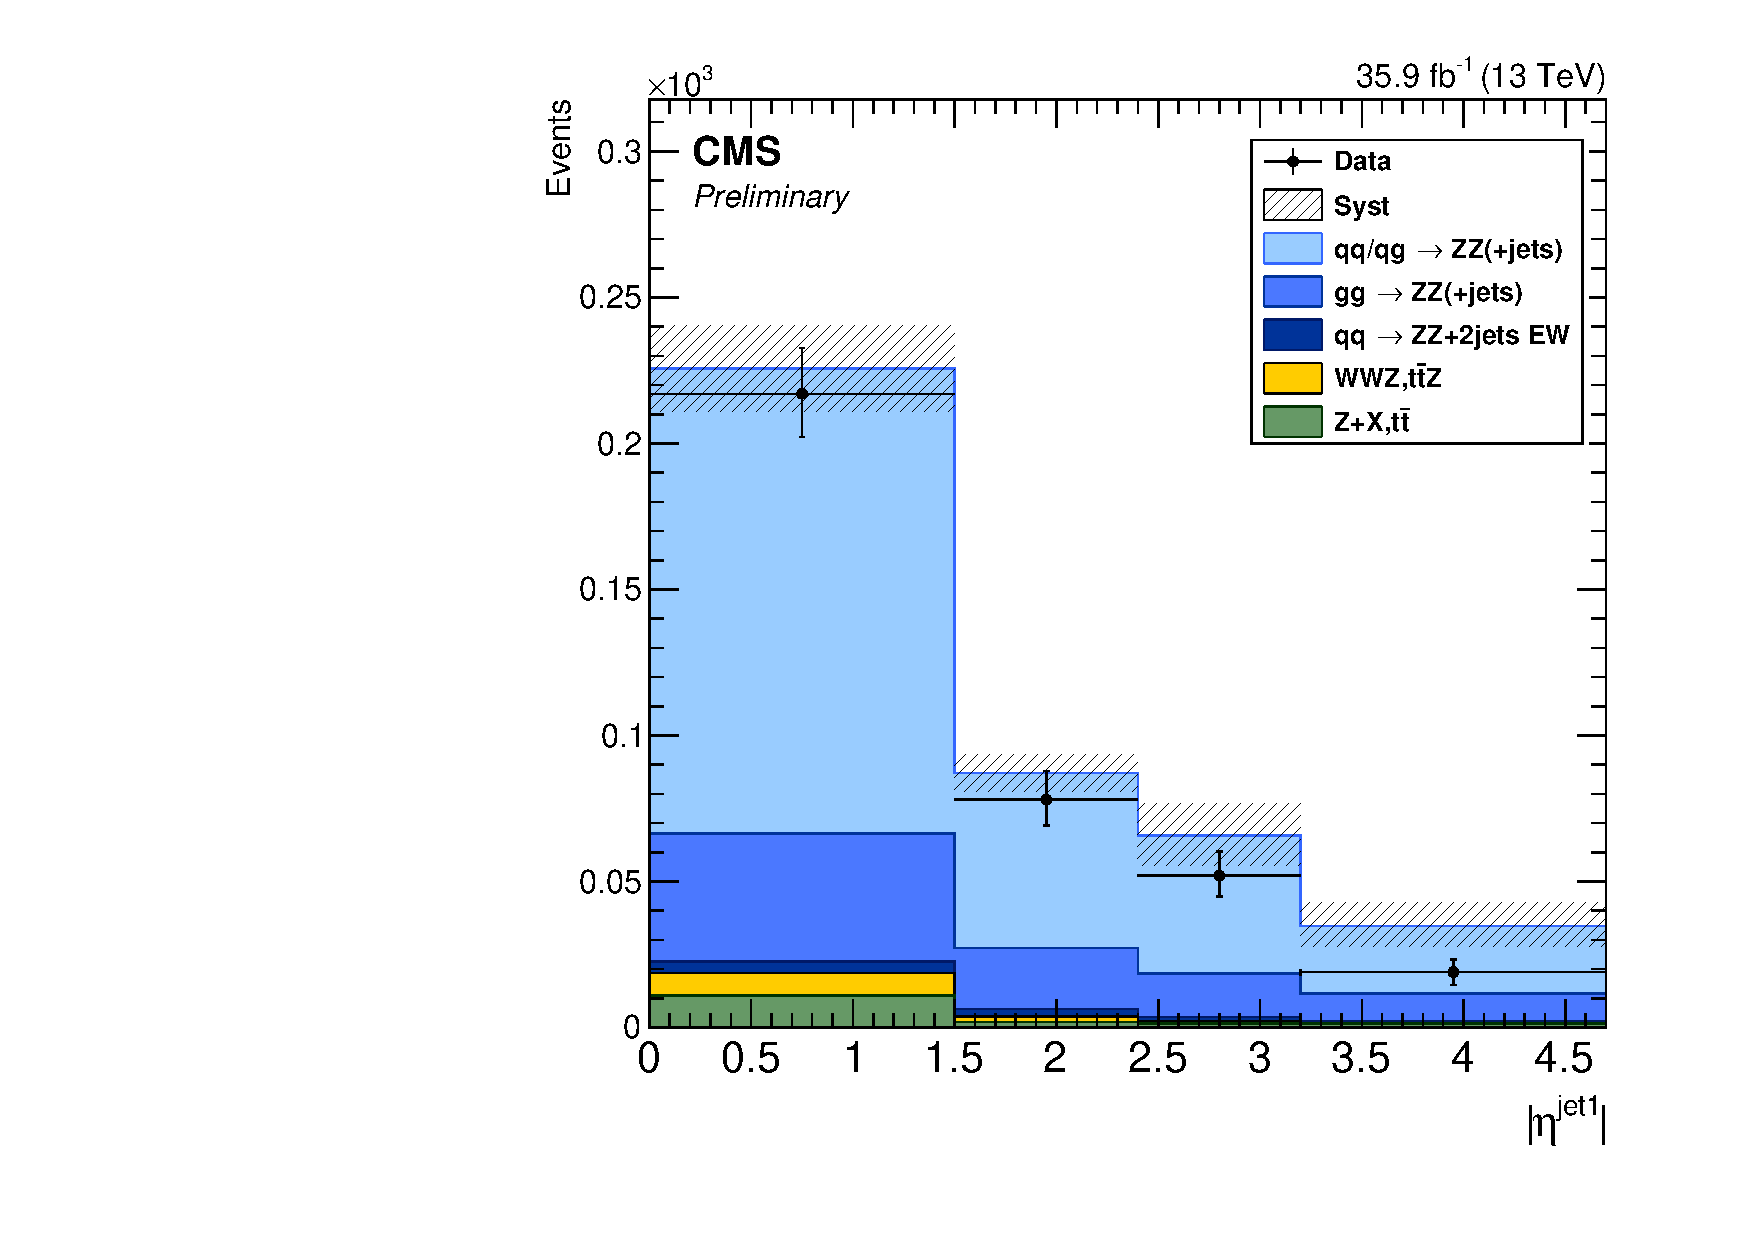
\includegraphics[width=0.48\textwidth]{results/j1Eta.pdf}
    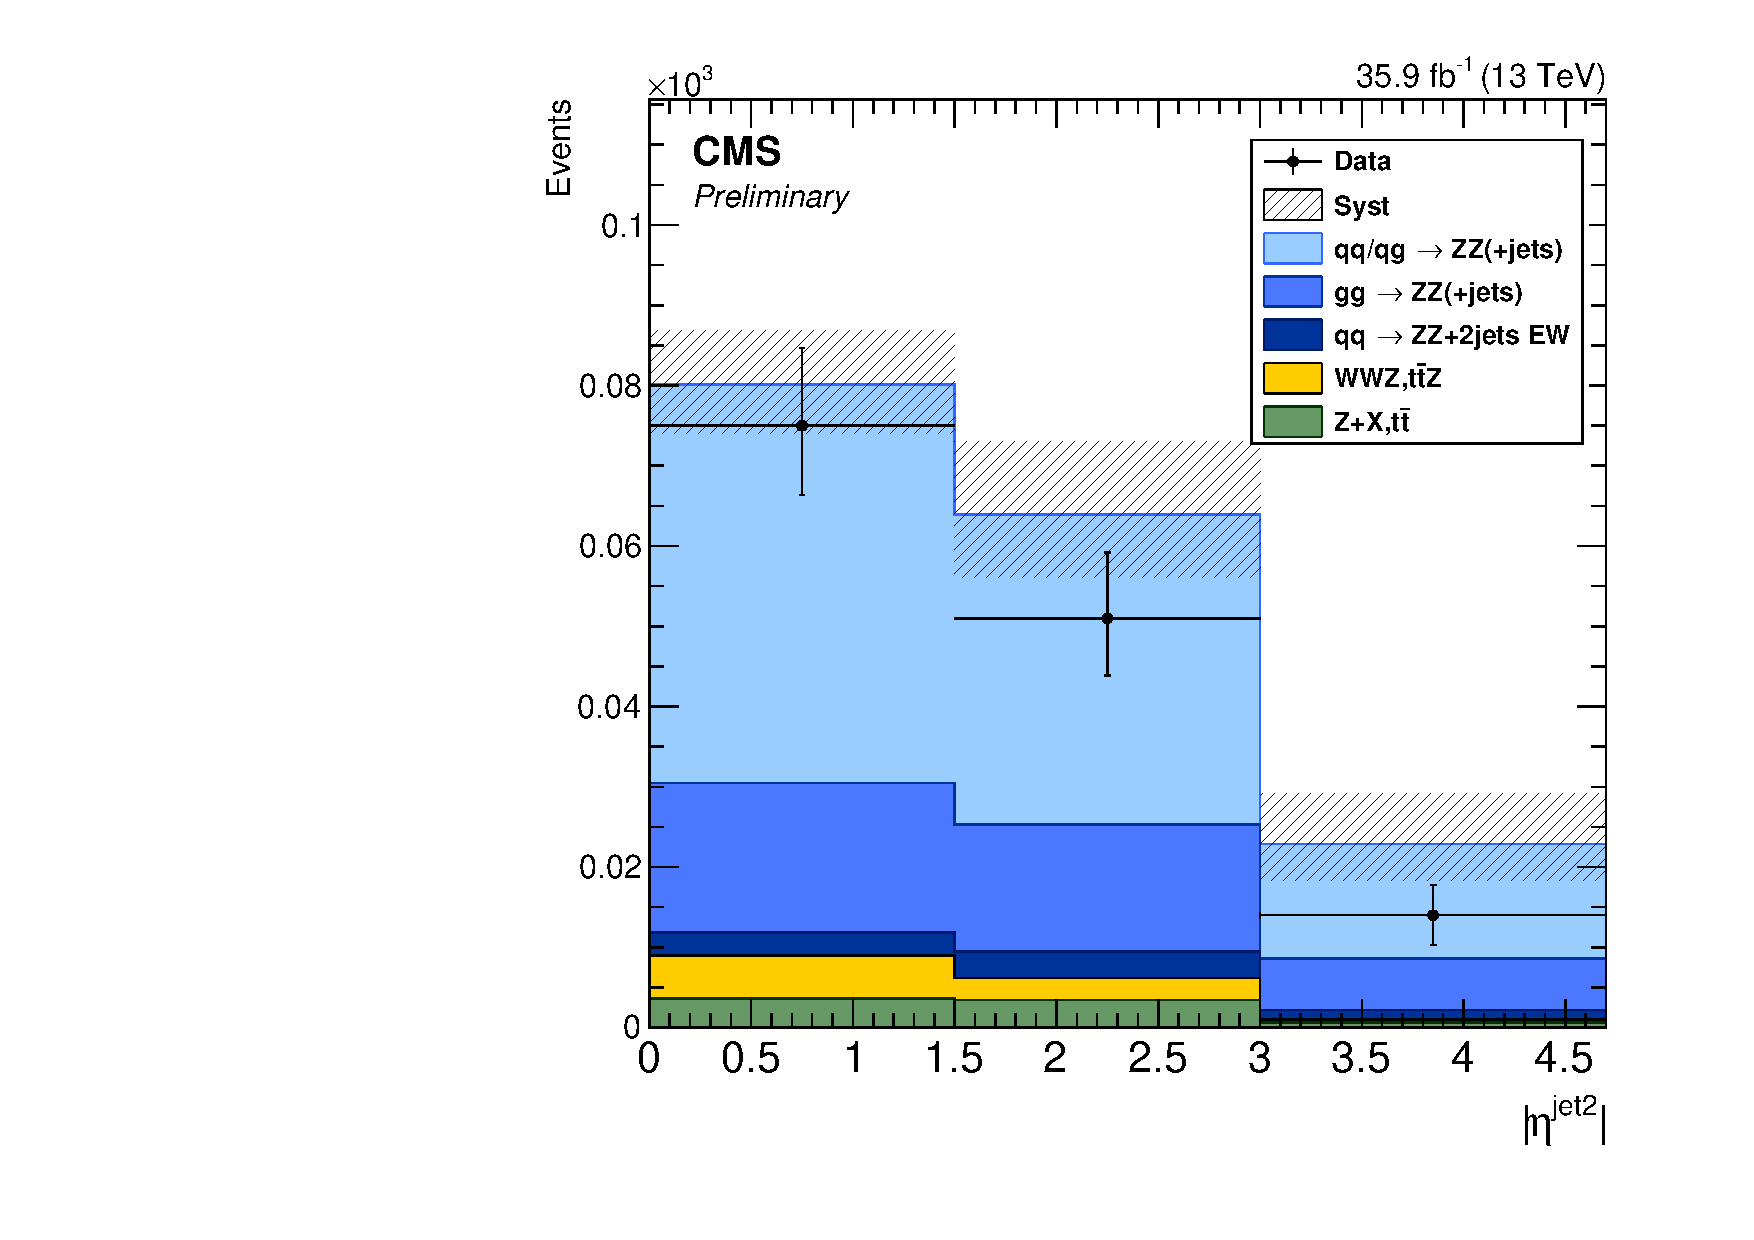
\includegraphics[width=0.48\textwidth]{results/j2Eta.pdf}
    \caption[Pseudorapidity of the leading and subleading jets]{
        Distribution of leading (left) and subleading (right) jet {\abseta} in {\ZZ} events with at least one jet and at least two jets, respectively.
        Points represent data, with statistical uncertainty bars.
        The stack of filled histograms represents the SM signal prediction and background estimate, with a hatched band showing the sum in quadrature of the statistical and systematic uncertainties on the total expected yield.
      }\label{fig:jetEta}
  \end{center}
\end{figure}

\begin{figure}[htbp]
  \begin{center}
    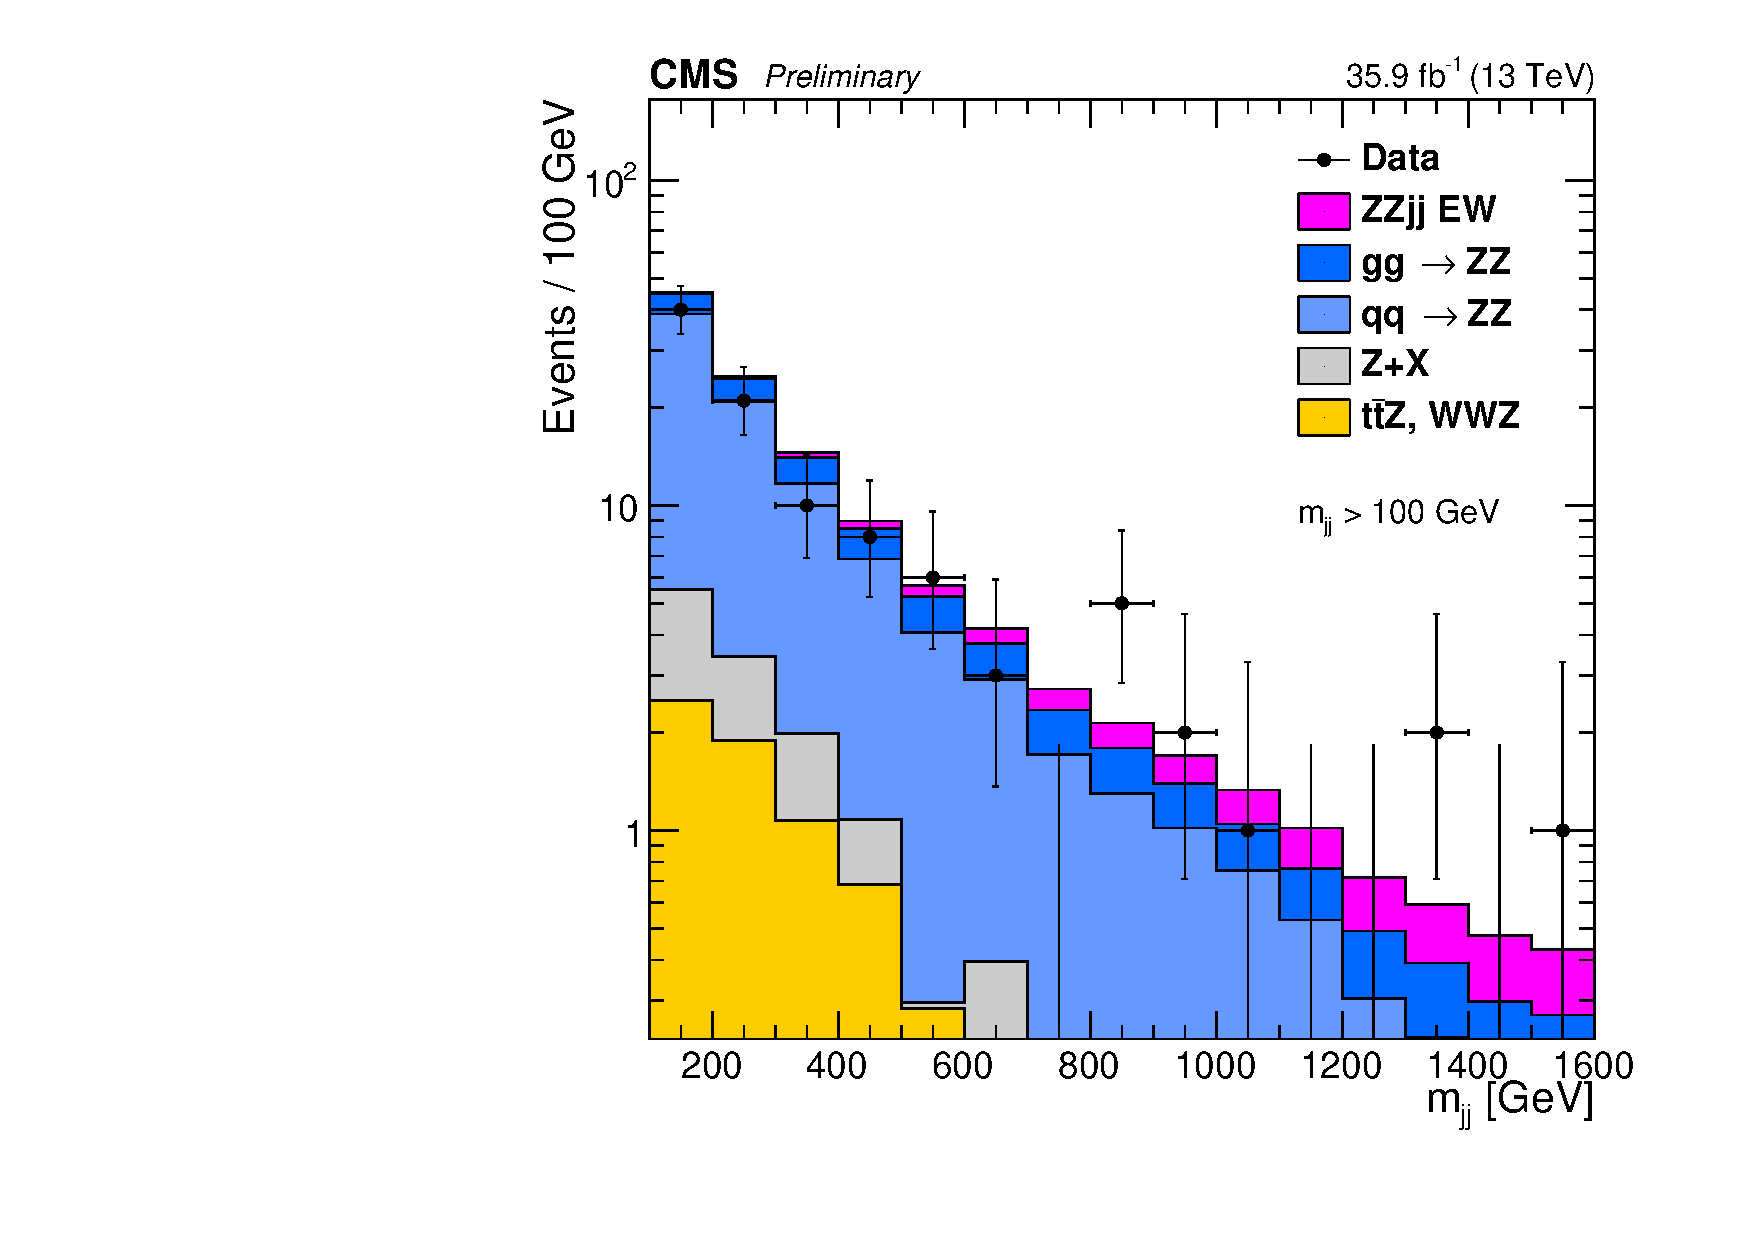
\includegraphics[width=0.75\textwidth]{results/mjj.pdf}
    \caption[Dijet invariant mass]{
        Dijet invariant mass $m_{\Pj\Pj}$ of the tag jets in {\ZZ} events passing the dijet selection.
        Points represent data, with statistical uncertainty bars.
        The stack of filled histograms represents the SM signal prediction and background estimate.
      }\label{fig:mjj}
  \end{center}
\end{figure}

\begin{figure}[htbp]
  \begin{center}
    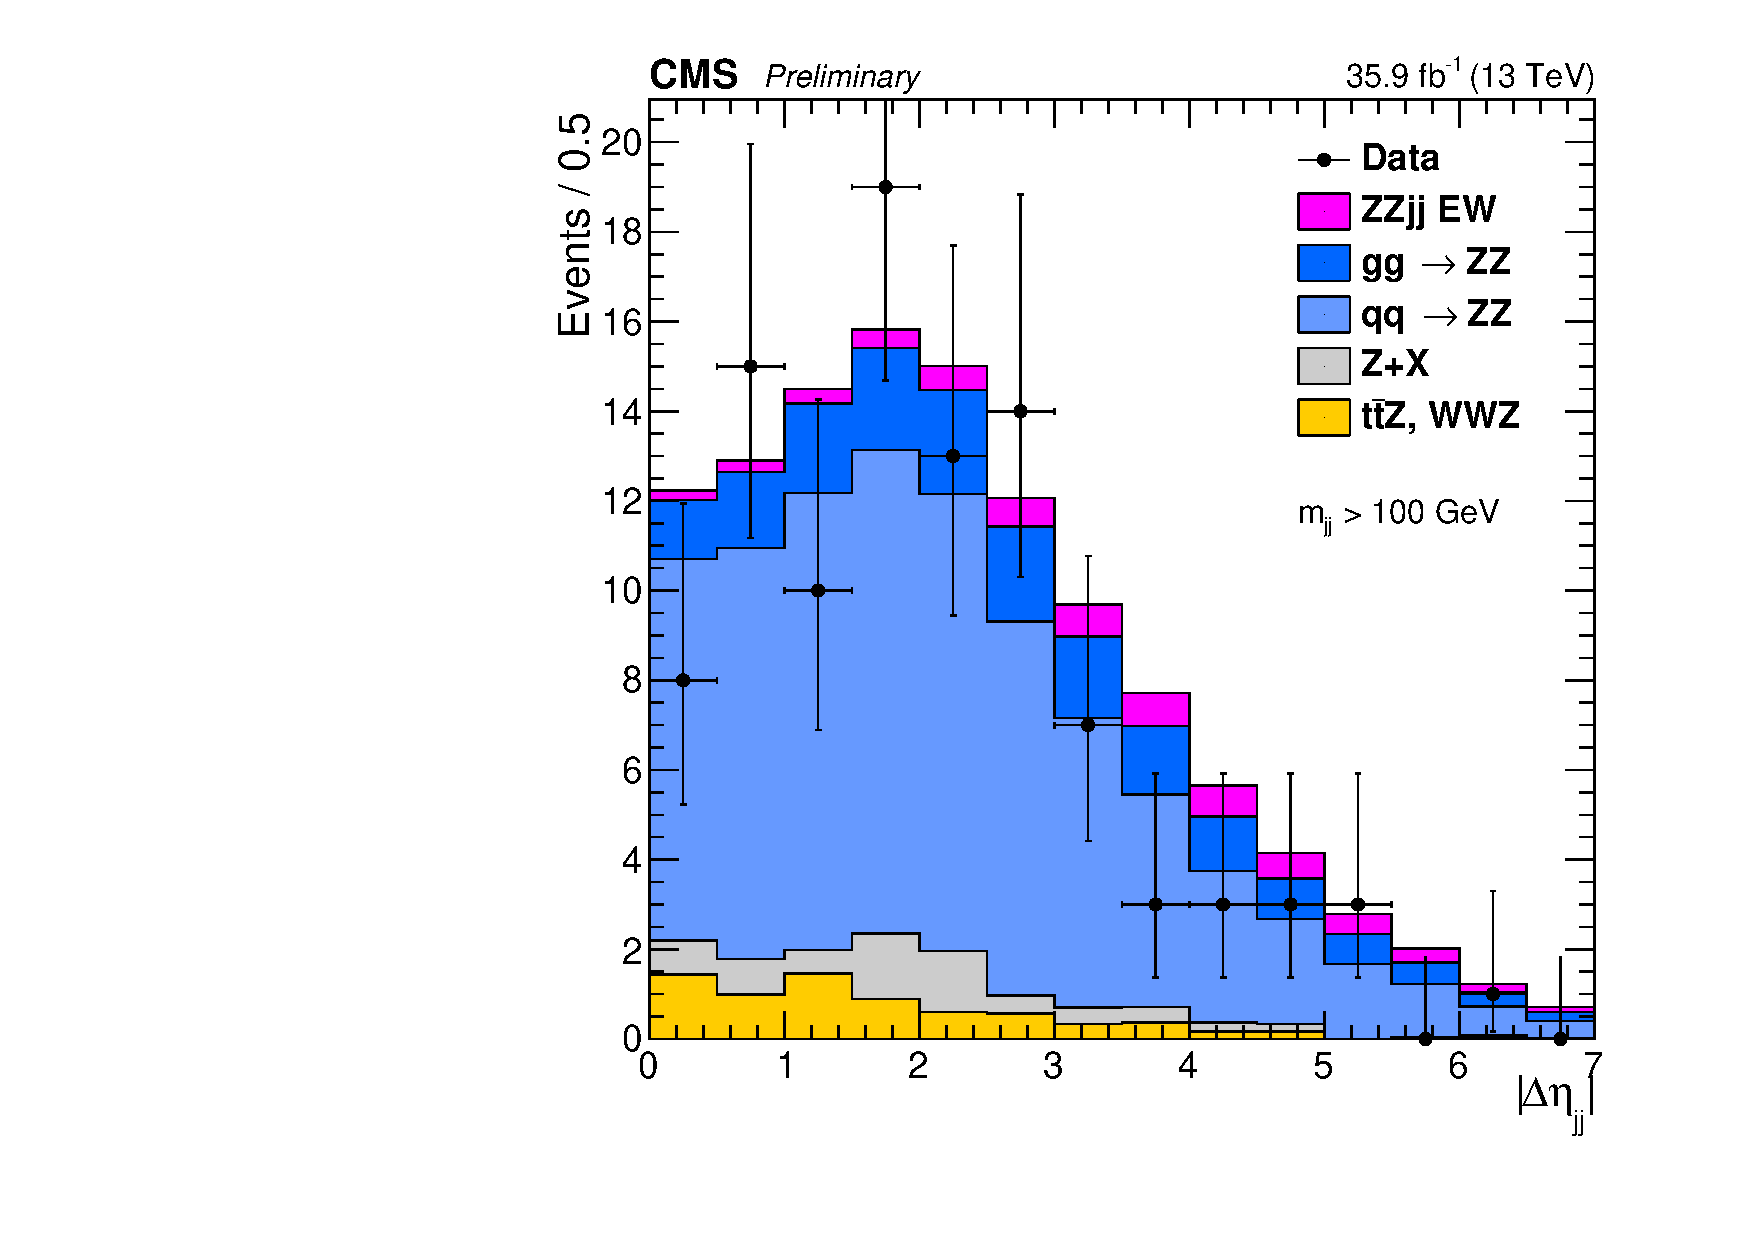
\includegraphics[width=0.75\textwidth]{results/deltaEtajj.pdf}
    \caption[Dijet pseudorapidity separation]{
        Pseudorapidity separation $\lvert \Delta \eta_{\Pj\Pj} \rvert$ of tag jets in {\ZZ} events passing the dijet selection.
        Points represent data, with statistical uncertainty bars.
        The stack of filled histograms represents the SM signal prediction and background estimate.
      }\label{fig:deltaEtajj}
  \end{center}
\end{figure}


\section{ZZ Fiducial and Total Cross Section}

The yields shown in Table~\ref{tab:results_zz} and the systematic uncertainties of Table~\ref{tab:systematics} are used as inputs to the maximum likelihood method described in Section~\ref{sec:signalStrength} to obtain the on-shell {\ZZ} signal strength across all channels,
\begin{equation}
  \mu = 1.040 _{-0.032}^{+0.033} \stat _{-0.035}^{+0.037} \syst \pm 0.026 \lum,
\end{equation}
which gives a fiducial cross section
\begin{equation}
  \sigma_\text{fid} (\pp \to \ZZ \to 4\ell) = 40.9 \pm 1.3 \stat \pm 1.4 \syst \pm 1.0 \lum \unit{fb},
\end{equation}
in the {\ZZfourl} fiducial phase space of Table~\ref{tab:fiducialDefs}.
The corresponding total cross section is
\begin{equation}
  \sigma(\pp \to \ZZ) = 17.5 _{-0.5}^{+0.6} \stat \pm 0.6 \syst \pm 0.4 \thy \pm 0.4 \lum \unit{pb}.
\end{equation}

This measurement, on 2016 data, agrees with the 2015 measurement~\cite{Khachatryan:2016txa}:
\begin{equation}
  \sigma(\pp \to \ZZ) = 14.6 ^{+1.9}_{-1.8} \stat _{-0.5}^{+0.3} \syst \pm 0.2 \thy \pm 0.4 \lum \unit{pb}.
\end{equation}
One may combine the measurements by doing a six-bin simultaneous fit with the 2015 and 2016 channels considered separate.
The degree of correlation between the systematic uncertainties in the 2015 and 2016 runs is not known, but the 2015 contribution is small enough that the systematic uncertainties are dominated by those in the 2016 dataset, and the degree of correlation will have only a small effect on the measurement.
We therefore do the fit twice, once treating the experimental uncertainties as fully correlated between the datasets, and again treating them as fully uncorrelated.
The small difference in the central value obtained is added linearly to the systematic error of the result.
After the full combination, the ``$2015 + 2016$'' total cross section is found to be
\begin{equation}
  \sigma(\pp \to \ZZ) = 17.2 \pm 0.5 \stat \pm 0.7 \syst \pm 0.4 \thy \pm 0.4 \lum \unit{pb}.
\end{equation}
These results can be compared to the {\MATRIX} prediction of $16.2^{0.6}_{-0.4}\unit{pb}$, computed at NNLO in QCD, or the {\MCFM} prediction of $15.0^{+0.7}_{-0.6} \pm 0.2\unit{pb}$, calculated at NLO in QCD with LO $\Pg\Pg \to \ZZ$ diagrams included.
Both predictions use the NNPDF3.0 PDF sets and fixed scales $\mu_\text{F} = \mu_\text{R} = m_\PZ$.

The total cross section is shown as a function of $\sqrt{s}$ in Fig.~\ref{fig:xsec_vs_sqrts}.
Measurements from CMS~\cite{Chatrchyan:2012sga,CMS:2014xja,Khachatryan:2015pba,Khachatryan:2016txa} and ATLAS~\cite{Aad:2012awa,Aad:2015rka,Aad:2015zqe} are compared to NLO predictions made with {\MCFM} (with contributions from leading order gluon-gluon fusion diagrams), and NNLO predictions made with {\MATRIX}.
Results from both experiments agree with the predictions.

\begin{figure}[htbp]
  \begin{center}
    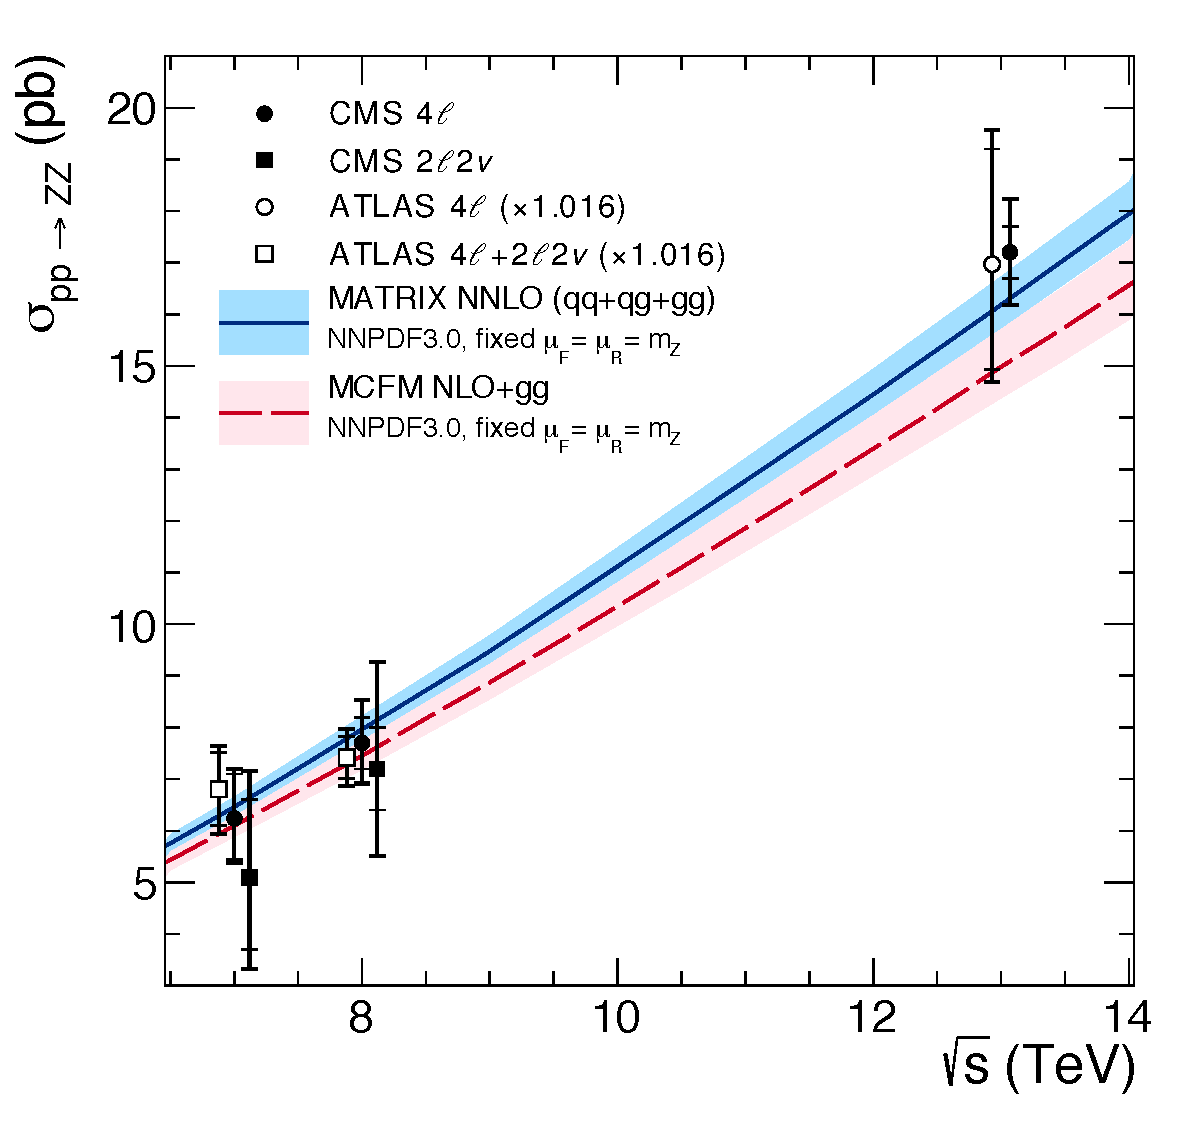
\includegraphics[width=0.95\textwidth]{results/sqrts.pdf}
    \caption[Total {\ZZ} cross section as a function of center-of-mass energy]{
        The total {\ZZ} cross section is shown as a function of $\sqrt{s}$.
        Measurements from CMS and ATLAS are both shown, with the ATLAS numbers adjusted upward by 1.6\% to account for differences in {\PZ} mass window choice.
        Points at the same center-of-mass energy as shifted slightly in the horizontal direction for clarity.
        Experimental measurements are compared to predictions from {\MCFM} at NLO in QCD with additional contributions from LO gluon-gluon fusion diagrams, and {\MATRIX} at NNLO in QCD\@.
        Both sets of predictions use the NNPDF3.0 PDF sets and fixed scales $\mu_\text{F} = \mu_\text{R} = m_\PZ$.
      }\label{fig:xsec_vs_sqrts}
  \end{center}
\end{figure}


\subsection[\texorpdfstring{$\mathrm{Z} \to 4\ell$}{Z to 4l} Branching  Fraction]{$\mathbf{Z} \to \mathbf{4\ell}$ Branching  Fraction}

The signal strength in the {\Zfourl} selection is
\begin{equation}
  \mu = 0.980 _{-0.044}^{+0.046} \stat _{-0.059}^{+0.065} \syst \pm 0.025 \lum,
\end{equation}
yielding a fiducial cross section
\begin{equation}
  \sigma_\text{fid}\left(\pp \to \PZ \to 4\ell\right) = 31.2 _{-1.4}^{+1.5} \stat _{-1.9}^{+2.1} \syst \pm 0.8 \lum \unit{fb}.
\end{equation}
This is scaled by an acceptance correction factor $\mathcal{A} = 0.125 \pm 0.002$, estimated with {\POWHEG}, to the total {\Zfourl} cross section times branching ratio,
\begin{equation}
  \sigma(\pp \to \PZ) \times \mathcal{B}(\PZ \to 4\ell) = 249 \pm 8 \stat ^{+9}_{-8} \syst \pm 4 \thy \pm 6 \lum \unit{fb}.
\end{equation}

Equation~\ref{eq:brCalc} is used to calculate the branching fraction.
The {\PZ} cross section times dilepton branching ratio is calculated with {\FEWZ}~v2.0~\cite{Gavin:2010az} at NNLO in QCD to be $1870 ^{+50}_{-40}\unit{pb}$.
A correction factor $\mathcal{C}^{\text{60--120}}_{\text{80--100}} = 0.926 \pm 0.001$, calculated with {\POWHEG}, is used to account for the difference in {\PZ} boson mass window between the measured {\Zfourl} cross section and the {\FEWZ} calculation.
Its uncertainty includes scale and PDF variations.
The nominal {\PZ} to dilepton branching fraction is $\mathcal{B}\left( \PZ \to 2\ell \right) = 0.03366$~\cite{Olive:2016xmw}.
The four-lepton branching fraction is measured to be
\begin{equation}
  \mathcal{B}\left(\Zfourl\right) = 4.8 \pm 0.2 \stat \pm 0.2 \syst \pm 0.1 \thy \pm 0.1 \lum \times 10^{-6}.
\end{equation}
This value is consistent with the theoretical value of $4.6 \times 10^{-6}$, calculated with {\MGAMC}, and with previous measurements from CMS and ATLAS~\cite{CMS:2012bw,Khachatryan:2016txa,Aad:2014wra}.



\section{Differential Cross Sections}

Detector-level distributions are unfolded to calculate differential cross sections as described in Section~\ref{sec:diffXSec}.
Dif

\begin{figure}[htbp]
  \begin{center}
    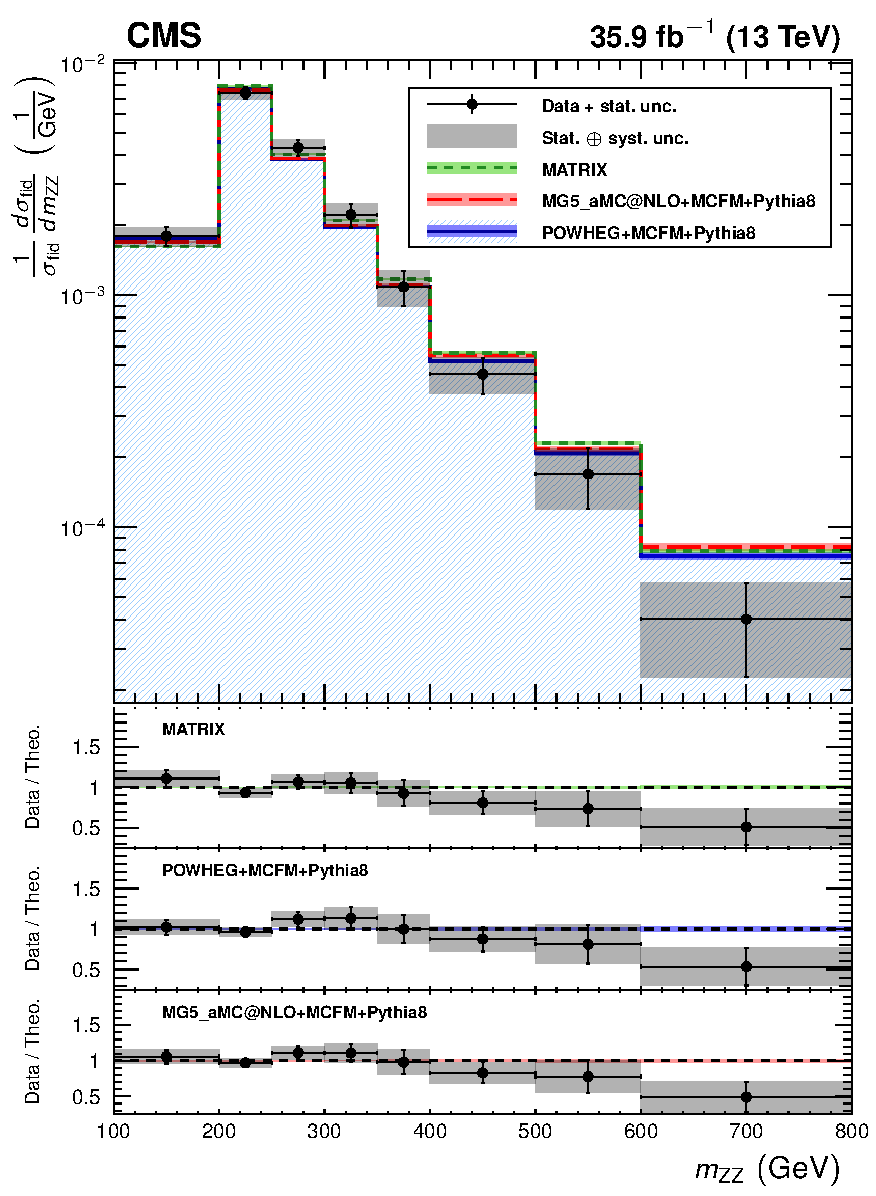
\includegraphics[width=0.8\textwidth]{results/unfold_mass.pdf}
    \caption[Normalized differential {\ZZ} cross section as a function of four-lepton invariant mass]{
        The {\ZZ} differential cross section as a function of $m_{4\ell}$, normalized to the total fiducial cross section.
        Points represent the unfolded data, with vertical bars showing the statistical uncertainty and a grey band showing the sum in quadrature of the statistical and systematic uncertainties.
        Blue, red, and green histograms represent the {\POWHEG}+{\MCFM}, {\MGAMC}+{\MCFM}, and {\MATRIX} predictions, with bands around each which represent their combined statistical, scale, and PDF uncertainties.
        The lower sections of the plot represents the ratio of the measured cross section to each of the predictions.
      }\label{fig:unfold_mass}
  \end{center}
\end{figure}

\begin{figure}[htbp]
  \begin{center}
    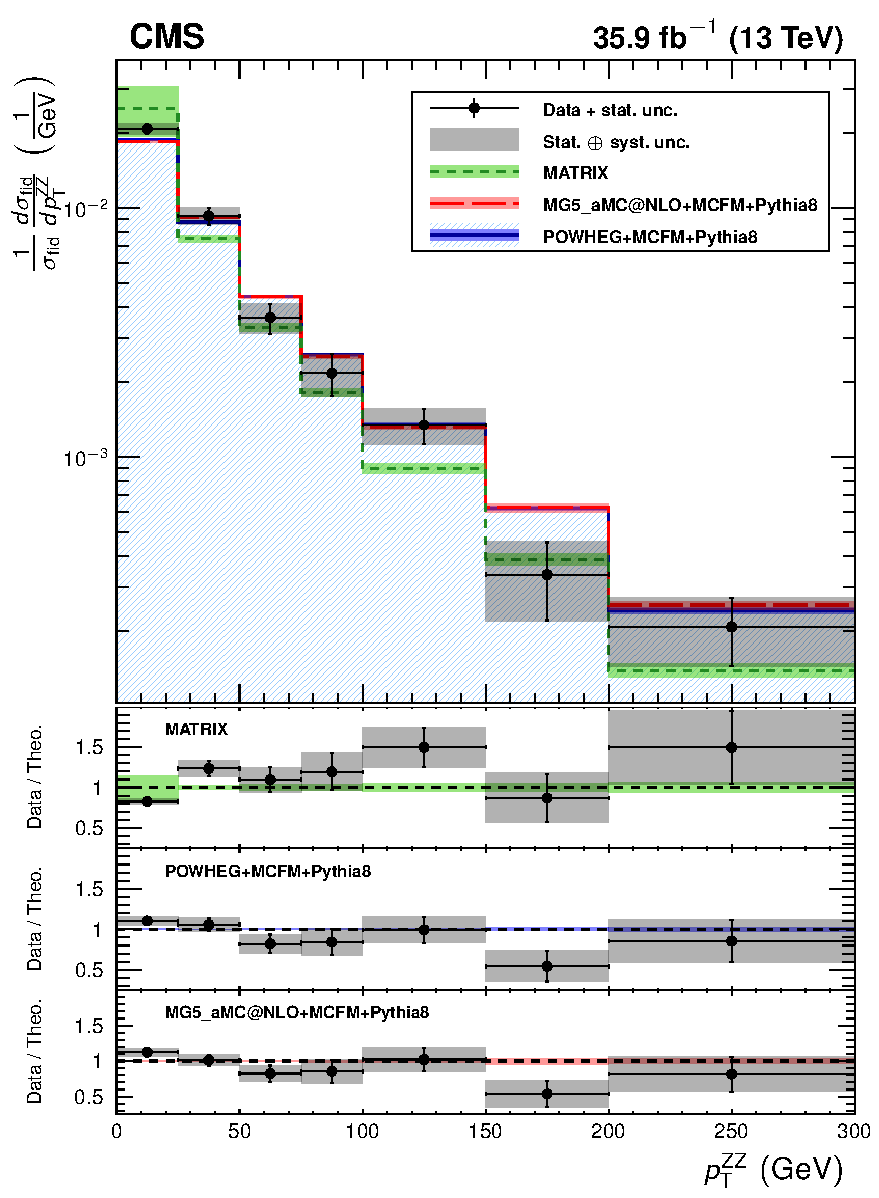
\includegraphics[width=0.8\textwidth]{results/unfold_pt.pdf}
    \caption[Normalized differential {\ZZ} cross section as a function of four-lepton system {\pt}]{
        The {\ZZ} differential cross section as a function of the four-lepton {\pt}, normalized to the total fiducial cross section.
        Points represent the unfolded data, with vertical bars showing the statistical uncertainty and a grey band showing the sum in quadrature of the statistical and systematic uncertainties.
        Blue, red, and green histograms represent the {\POWHEG}+{\MCFM}, {\MGAMC}+{\MCFM}, and {\MATRIX} predictions, with bands around each which represent their combined statistical, scale, and PDF uncertainties.
        The lower sections of the plot represents the ratio of the measured cross section to each of the predictions.
      }\label{fig:unfold_pt}
  \end{center}
\end{figure}

\begin{figure}[htbp]
  \begin{center}
    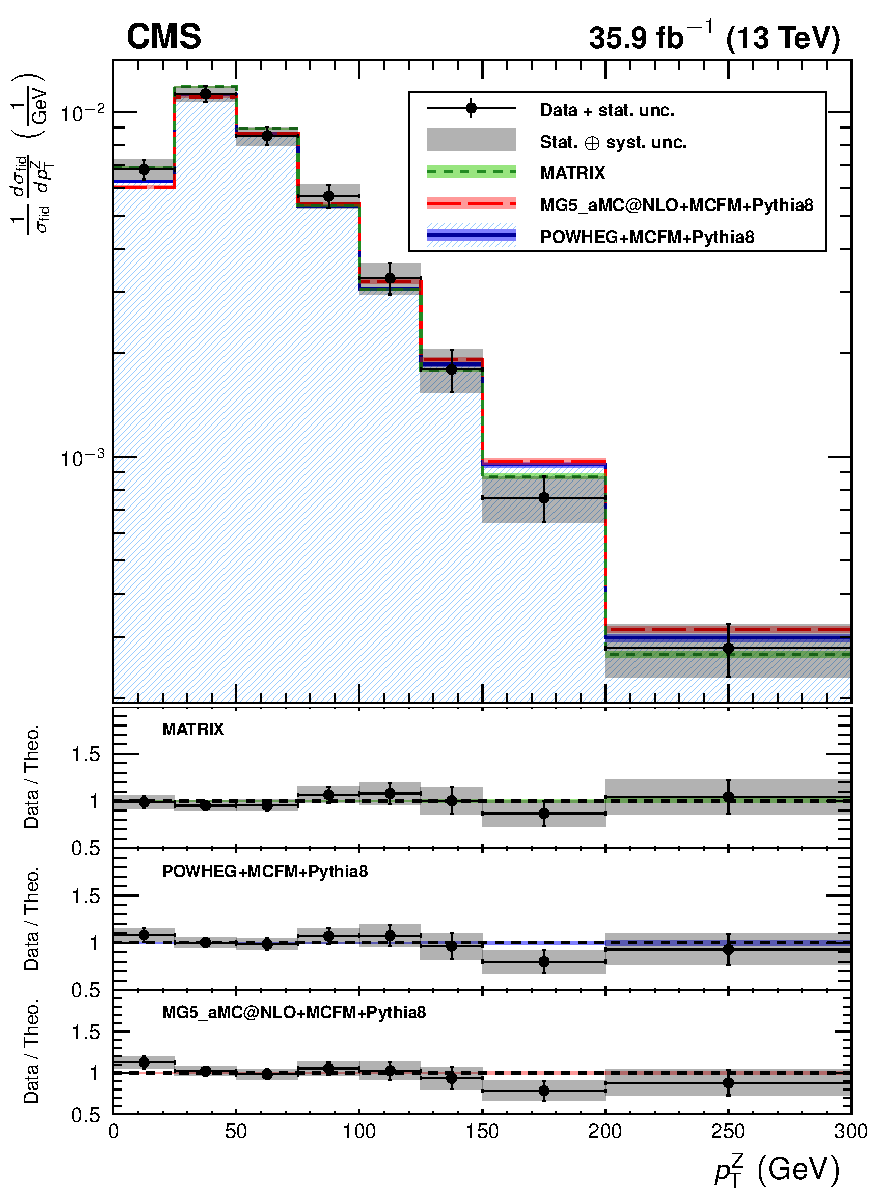
\includegraphics[width=0.8\textwidth]{results/unfold_zPt.pdf}
    \caption[Normalized differential {\ZZ} cross section as a function of {\PZ} boson candidate {\pt}]{
        The {\ZZ} differential cross section as a function of the {\pt} of both {\PZ} boson candidates, regardless of which one is $\PZ_1$ and which is $\PZ_2$, normalized to the total fiducial cross section.
        Points represent the unfolded data, with vertical bars showing the statistical uncertainty and a grey band showing the sum in quadrature of the statistical and systematic uncertainties.
        Blue, red, and green histograms represent the {\POWHEG}+{\MCFM}, {\MGAMC}+{\MCFM}, and {\MATRIX} predictions, with bands around each which represent their combined statistical, scale, and PDF uncertainties.
        The lower sections of the plot represents the ratio of the measured cross section to each of the predictions.
      }\label{fig:unfold_zPt}
  \end{center}
\end{figure}

\begin{figure}[htbp]
  \begin{center}
    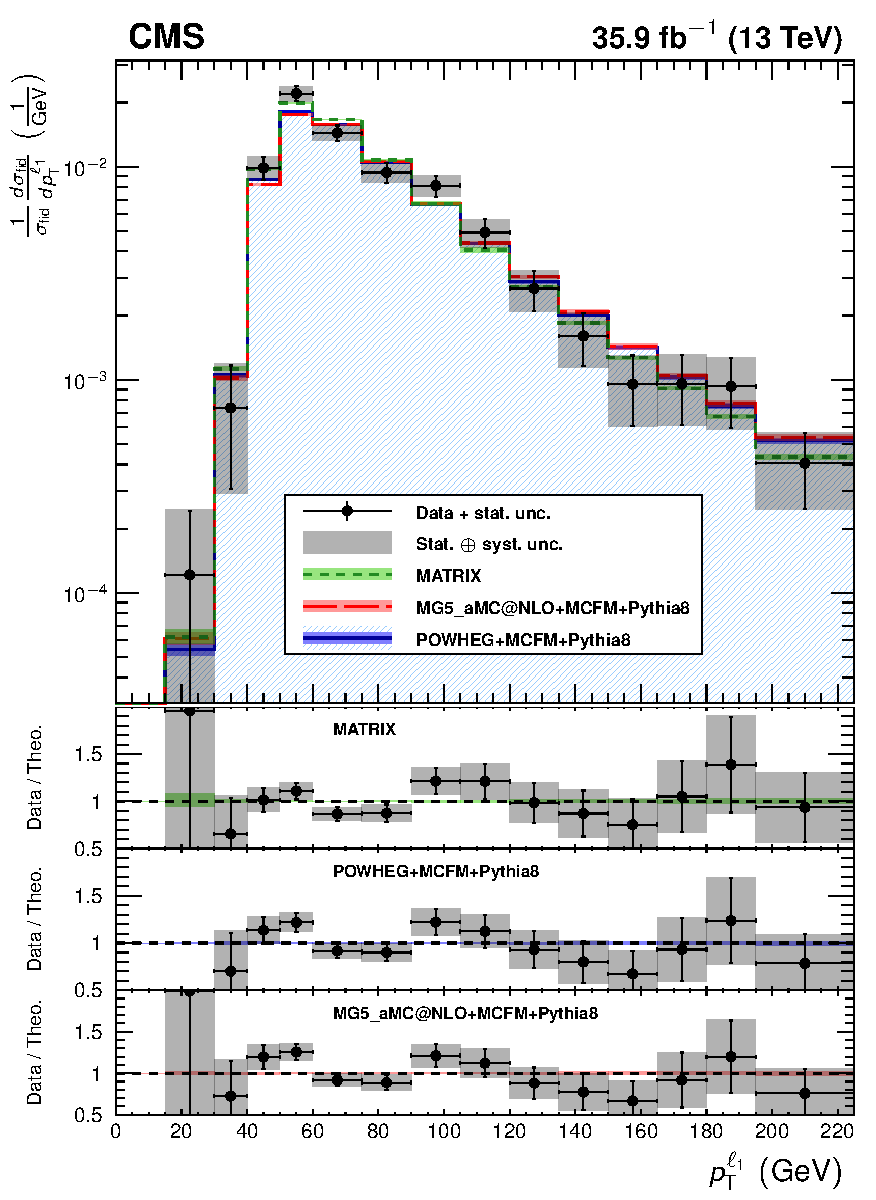
\includegraphics[width=0.8\textwidth]{results/unfold_l1Pt.pdf}
    \caption[Normalized differential {\ZZ} cross section as a function of leading lepton {\pt}]{
        The {\ZZ} differential cross section as a function of leading lepton {\pt}, normalized to the total fiducial cross section.
        Points represent the unfolded data, with vertical bars showing the statistical uncertainty and a grey band showing the sum in quadrature of the statistical and systematic uncertainties.
        Blue, red, and green histograms represent the {\POWHEG}+{\MCFM}, {\MGAMC}+{\MCFM}, and {\MATRIX} predictions, with bands around each which represent their combined statistical, scale, and PDF uncertainties.
        The lower sections of the plot represents the ratio of the measured cross section to each of the predictions.
      }\label{fig:unfold_l1Pt}
  \end{center}
\end{figure}

\begin{figure}[htbp]
  \begin{center}
    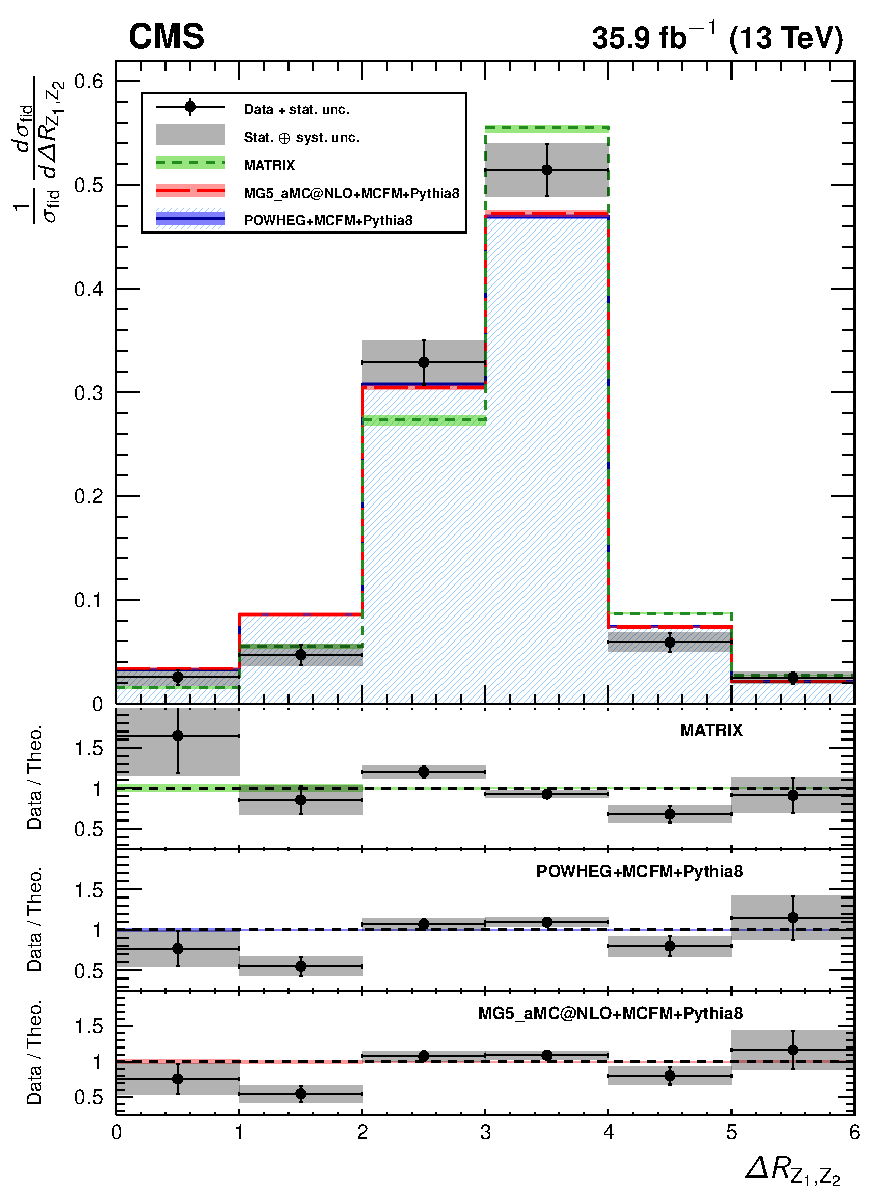
\includegraphics[width=0.8\textwidth]{results/unfold_deltaRZZ.pdf}
    \caption[Normalized differential {\ZZ} cross section as a function of $\Delta R$ between the {\PZ} bosons]{
        The {\ZZ} differential cross section as a function of $\Delta R$ between the two {\PZ} bosons, normalized to the total fiducial cross section.
        Points represent the unfolded data, with vertical bars showing the statistical uncertainty and a grey band showing the sum in quadrature of the statistical and systematic uncertainties.
        Blue, red, and green histograms represent the {\POWHEG}+{\MCFM}, {\MGAMC}+{\MCFM}, and {\MATRIX} predictions, with bands around each which represent their combined statistical, scale, and PDF uncertainties.
        The lower sections of the plot represents the ratio of the measured cross section to each of the predictions.
      }\label{fig:unfold_deltaRZZ}
  \end{center}
\end{figure}

\begin{figure}[htbp]
  \begin{center}
    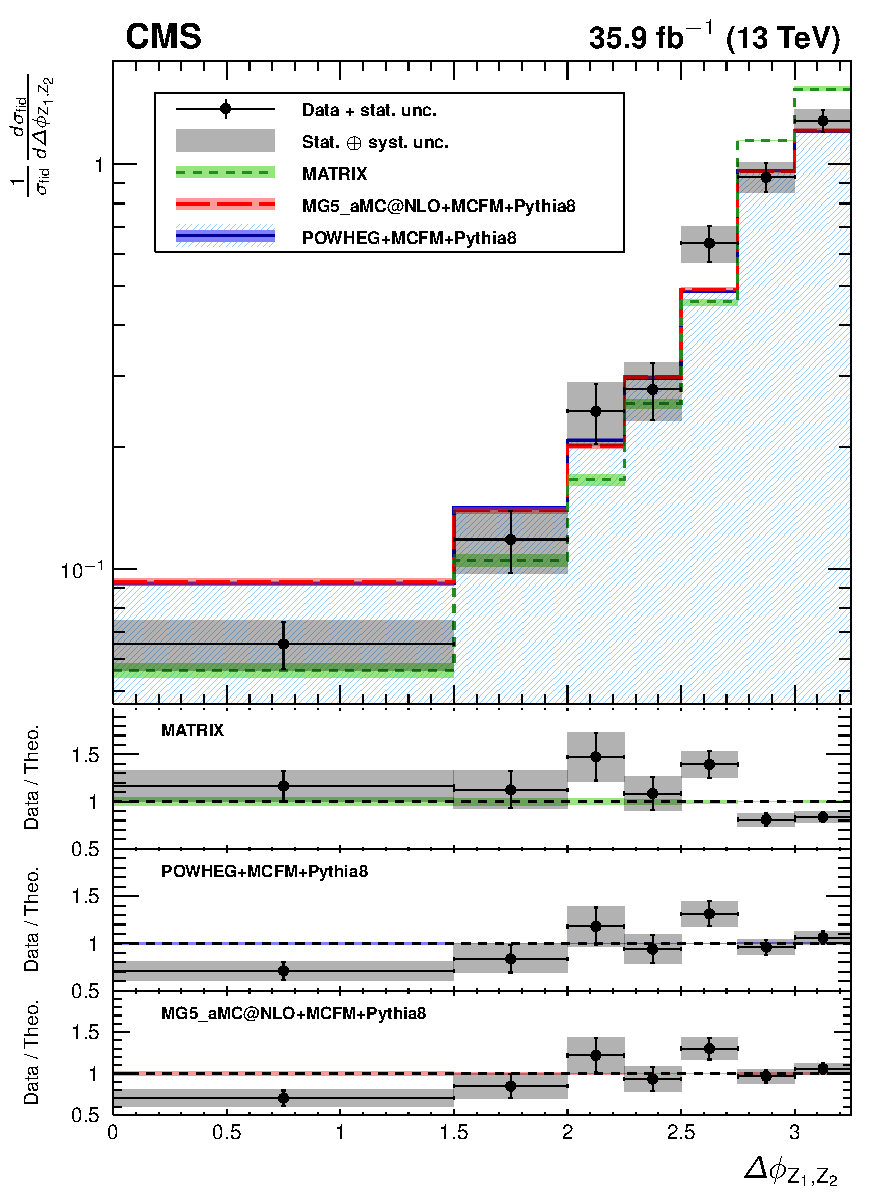
\includegraphics[width=0.8\textwidth]{results/unfold_deltaPhiZZ.pdf}
    \caption[Normalized differential {\ZZ} cross section as a function of $\Delta \phi$ between the {\PZ} bosons]{
        The {\ZZ} differential cross section as a function of $\Delta \phi$ between the two {\PZ} bosons, normalized to the total fiducial cross section.
        Points represent the unfolded data, with vertical bars showing the statistical uncertainty and a grey band showing the sum in quadrature of the statistical and systematic uncertainties.
        Blue, red, and green histograms represent the {\POWHEG}+{\MCFM}, {\MGAMC}+{\MCFM}, and {\MATRIX} predictions, with bands around each which represent their combined statistical, scale, and PDF uncertainties.
        The lower sections of the plot represents the ratio of the measured cross section to each of the predictions.
      }\label{fig:unfold_deltaPhiZZ}
  \end{center}
\end{figure}

\begin{figure}[htbp]
  \begin{center}
    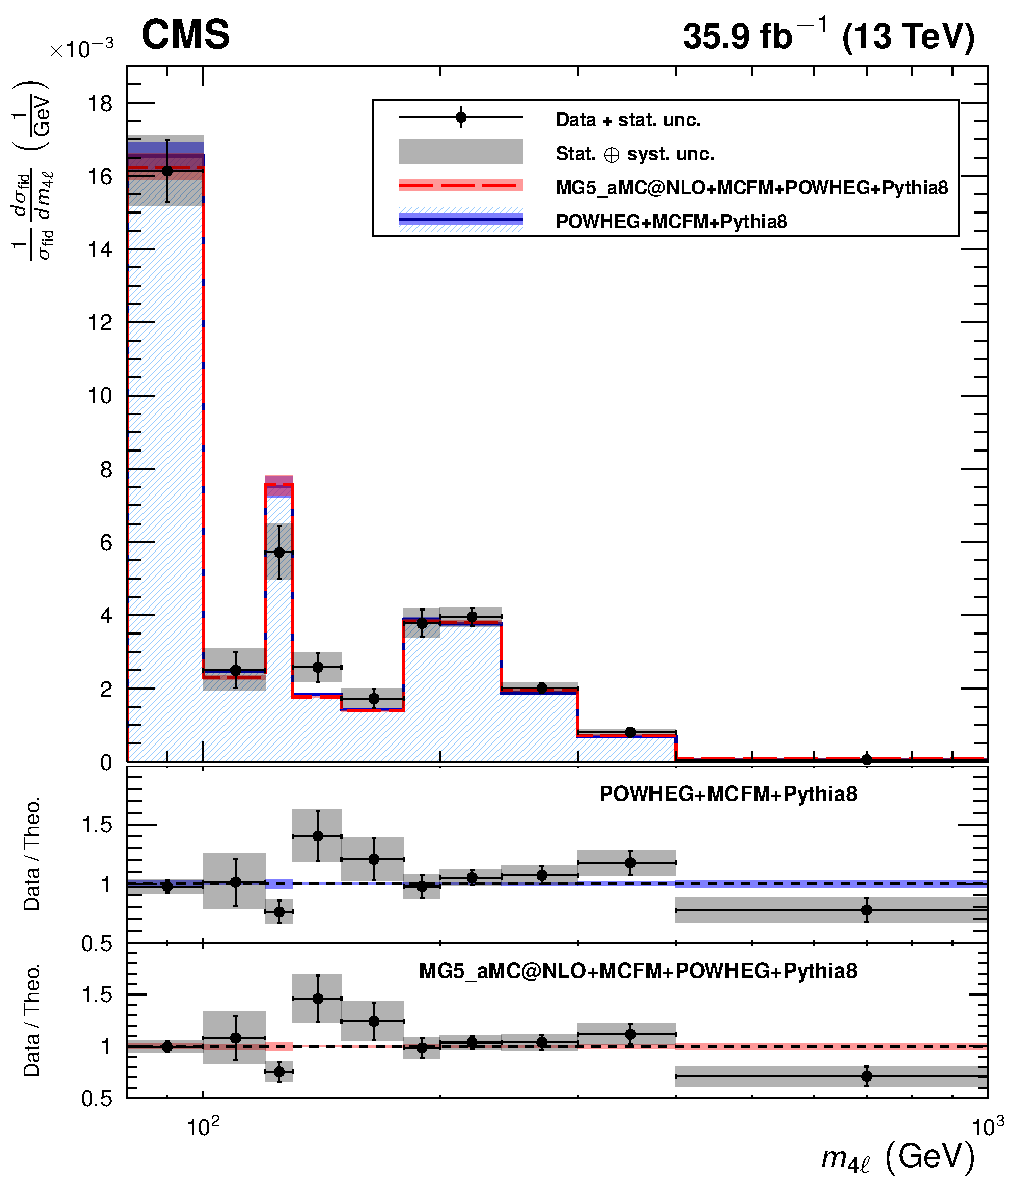
\includegraphics[width=0.8\textwidth]{results/unfold_massFull.pdf}
    \caption[Normalized differential four-lepton cross section as a function of four-lepton invariant mass with loosened {\PZ} mass cuts]{
        The four-lepton differential cross section as a function of $m_{4\ell}$ under the full spectrum selections, normalized to the total fiducial cross section.
        Points represent the unfolded data, with vertical bars showing the statistical uncertainty and a grey band showing the sum in quadrature of the statistical and systematic uncertainties.
        Blue and red histograms represent the {\POWHEG}+{\MCFM} and {\MGAMC}+{\MCFM} predictions, with bands around each which represent their combined statistical, scale, and PDF uncertainties.
        The lower sections of the plot represents the ratio of the measured cross section to each of the predictions.
      }\label{fig:unfold_massFull}
  \end{center}
\end{figure}



\section{Vector Boson Scattering}
Electroweak signal's electrostrength



\section{Anomalous Coupling Limits}
Winning at not finding things
